\chapter{Diversité de l'architecture génomique chez les bactéries}\label{chap1a}
\lhead{\emph{Diversité de l'architecture génomique chez les bactéries}}


Ce chapitre a pour objectif de détailler le contexte biologique et génomique de l'étude à partir de la littérature existante. Nous nous focaliserons cependant sur les mécanismes de réplication/ségrégation et maintenance du cycle cellulaire. Dans un deuxième temps, nous soulèverons la question de l'étude, nous détaillerons l'importance de celle-ci dans le contexte de la génomique évolutive et des potentielles implications sur la compréhension de l'évolution des génomes bactériens.


\section{Architecture génomique des trois domaines du vivant}
 
Tout organisme vivant est composé de cellule(s). L'information les définissant a pour support physique un génome, ensemble du matériel génétique, composé de molécule(s) d'acide désoxyribonucléique (ADN). L'information qu'il code, nécessaire au développement et au fonctionnement cellulaire, s'exprime non seulement dans la synthèse d'acide ribonucléique (ARN) et de protéines par l'intermédiaire du code génétique, mais aussi à travers l'organisation spatiale du génome. L'information codée permet de plus sa propre reproduction et, ainsi, assure la conservation du matériel génétique à travers le temps et les générations. Enfin, le génome permet l'évolution et l'adaptation d'une population par sa capacité à être modifié de génération en génération. Tous les organismes ne possèdent pas la même architecture génomique, celle-ci reflétant notamment des différences de morphologie et d'écologie des espèces.\\

Les organismes vivants sont classés en trois domaines: Archées, Eucaryotes et Bactéries. Les virus, parfois proposés comme quatrième domaine du vivant \citep{mcgeoch2008extra}, en sont néanmoins exclus actuellement car n'existant pas sous une forme cellulaire. Ces trois domaines se différencient par plusieurs propriétés essentielles (Table \ref{tabdomaincomp}) mais possèdent néanmoins des constituants génétiques similaires ainsi que les mêmes schémas fonctionnel et organisationnel fondamentaux.


\begin{table}[H]\label{tabdomaincomp}
\begin{center}
\caption[Comparaison des structures génomiques des trois domaines du vivant]{Comparaison des structures génomiques des trois domaines du vivant. Adapté de \citep{perry1997microbiology} }\label{tabdomaincomp}
\begin{tabular}{cccc}
	\textbf{Caractéristiques} & Bactéries & Archées & Eucaryotes\\
	\hline
	\textbf{Génome} & & & \\
	Noyau & - & - & + \\
	Gyrase inverse & - & + & - \\
	\\
	\textbf{ARN} & & & \\
	Polymérase simple & + & - & - \\
	Polymérase complexe & - & + & - \\
	Polymérases multiples & - & - & + \\
	ARNm polycistronique & - & - & + \\
	Ribosomes 70S & + & + & +/- \\
	\\
	\textbf{Introns} & & & \\
	ARNt & - & +/- & + \\
	ARNr & +/- & +/- & - \\
	ARNm & +/- & +/- & - \\
\end{tabular} 
\end{center}
\end{table} 
 
 
 \section{Architecture génomique bactérienne: les réplicons}\label{architecture}
	Dans la compréhension de l'architecture des génomes, le terme de \textbf{réplicon} désigne une unité réplicative du génome. Ce terme a été introduit en 1963 \citep{jacob1963regulation} et désigne de façon générale une unité de réplication indépendante se répliquant dans son ensemble. D'un point de vue structural, un réplicon est l'élément génétique défini entre une origine de réplication active et un site de terminaison (Figure \ref{figreplintro}). 

\begin{figure}[H]
	\begin{center}
	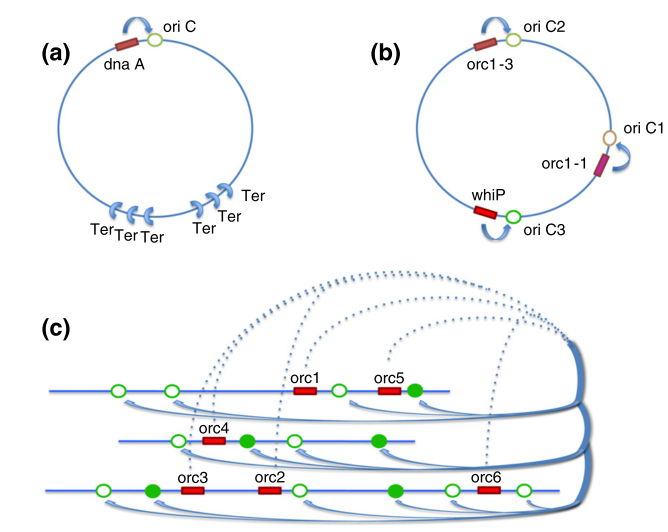
\includegraphics[height=0.4\textheight]{./img/replicon_diversification.png}
	\caption[Diversité des réplicons des trois domaines du vivant]{Diversité des réplicons des trois domaines du vivant. (a) Chromosome bactérien type avec une unique origine de réplication (\textit{ori}) et un site de terminaison à l'opposé. (b) Réplicon de type archée avec plusieurs \textit{ori} inspiré du génome de \textit{Sulfolobus islandicus}. (c) Génome eucaryote typique à multiples origines de réplication ORC. Tiré de \citep{hyrien2013simple}.}\label{figreplintro}
	 \end{center}
 \end{figure} 

	Différents réplicons peuvent être présents sur une même molécule d'ADN, ce qui est le cas général chez les Eucaryotes et semble être fréquent chez Archées \citep{samson2011cell}, cette configuration permettant alors de multiples amorçages de l'initiation de la réplication. Dans ce cas, il n'existe pas de site de terminaison précis. Chez les bactéries par contre, il est communément admis que chaque molécule d'ADN possède un unique réplicon actif.
Dans l'étude du génome d'\textit{Escherichia coli}, un des principaux et premiers organismes modèles en biologie, l'initiation de la réplication du génome, constitué d'un unique chromosome circulaire, s'effectue à un seul site, correspondant à la séquence d'origine de réplication ou \textbf{\textit{ori}} \citep{skarstad1986timing}. Ce phénomène, étant observé chez d'autres espèces bactériennes ainsi que pour des plasmides (voir ci-dessous) \citep{Messer2002,worning2006origin}, le terme ``réplicon" a été généralisé pour désigner, chez les bactéries, les différentes entités génomiques composées d'une unique molécule d'ADN. Quelques exceptions existent toutefois dans le cas des plasmides bactériens. Par exemple, des plasmides tels que les plasmides pGSH500 et pJD4 de \textit{Klebsiella pneumoniae} et \textit{Neisseria gonorrhoeae} respectivement, possèdent plusieurs \textit{ori} (réplicons \textit{sensu stricto}), ce qui leur permet de mieux s'intégrer dans le génome de multiples hôtes \citep{Toukdarian2004}.
 
 
 \subsection{Réplicons essentiels et accessoires}\label{essacc}
Le génome bactérien est constitué de réplicons essentiels à la survie des cellules, les chromosomes, et de réplicons non essentiels, les plasmides \citep{Mackenzie2004}. Historiquement, le terme de "plasmide" a été introduit par Lederberg en 1952 \citep{lederberg1952cell} et désignait à l'époque toute particule extra-chromosomique capable de se reproduire dans un état autonome. Cette définition englobait en fait ce que l'on désigne aujourd'hui sous les termes de ``virus", ``bactériophage", ``ribosome", ``transposon", ``séquence d'insertion" en plus de la définition actuelle de ``plasmide" \citep{lederberg1952cell}. Comment alors définir proprement un plasmide? Par opposition à un chromosome et aux autres éléments extra-chromosomiques, un plasmide peut être caractérisé par son spectre d'hôtes, son mode de réplication plus ou moins autonome vis-à-vis du génome de l'espèce hôte, sa capacité de mobilité inter-hôte, et par des mécanismes d'incompatibilité inter-plasmidique \citep{Slater2008,helinski2004introduction}. Les plasmides diffèrent des chromosomes en présentant des très hauts taux de flux génétiques, et peuvent porter des éléments génétiques provenant de bactéries qui n'ont pas ou peu de caractéristiques en commun. Les plasmides peuvent donc être vus comme des mosaïques de modules fonctionnels aux origines phylogéniques diverses \citep{Fernandez-Lopez2006}.\\
	La notion d'essentialité pour un réplicon est cependant ambiguë, dans le sens où un réplicon peut être qualifié d'essentiel si et seulement si il comporte au moins un gène essentiel à la survie de l'organisme \citep{Mackenzie2004}. Des marqueurs traditionnellement utilisés pour déterminer l'essentialité d'un réplicon sont les gènes codant les ARN ribosomiques (ARNr) \citep{Mackenzie2004}. L'étude de génomes réduits a fourni différents ensembles de gènes considérés comme étant essentiels à la survie des organismes bactériens \citep{Glass2006,Koonin2000}, qui peuvent être, de même, utilisés comme marqueurs d'essentialité de l'élément génétique. Mesurer l'essentialité d'un gène est cependant une tâche ardue en pratique. Elle dépend souvent de l'écologie de l'organisme et peut varier, pour un gène donné, d'un organisme à un autre. Enfin, dans certaines conditions, la perturbation d'un gène peut gravement entraver la capacité d'un organisme à se développer et à prospérer sans forcément le tuer \citep{Mackenzie2004,Slater2008}. Doit-on alors trancher sur le statut ``essentiel" ou ``accessoire" d'un gène donné selon la survie de l'organisme en cas d'altération du géne, ou peut-on plutôt parler de différents degrés d'essentialité d'un gène, et par extension d'un réplicon, selon l'organisme considéré?
 
 
 \subsection{Distribution des réplicons}
Le génome d'\textit{E. coli}, espèce modèle de référence, est composé d'un large réplicon: le chromosome et, selon les souches, de réplicons plasmidiques additionnels plus petits. Ce schéma est largement retrouvé parmi les bactéries. \textbf{La structure typique des génomes bactériens est donc: un unique chromosome, coexistant éventuellement avec des plasmides.} Cette constatation a été largement utilisée afin de décrire les génomes bactériens: le réplicon le plus large étant généralement désigné comme le chromosome et considéré comme essentiel, et les réplicons additionnels étant considérés comme des plasmides, donc accessoires \citep{casjens1998diverse}. Néanmoins, de nombreuses exceptions existent au sein des génomes bactériens (ces éléments seront approfondis dans le Chapitre \ref{chap1b}), ce qui remet en cause ce paradigme. 


\subsection{Taille des réplicons}
	Les réplicons bactériens présentent une très grande diversité de taille. Pour les chromosomes et réplicons extra-chromosomiques dont les séquences complètes étaient disponibles dans la base de données publiques RefSeq à la date du 23 octobre 2013, la taille des chromosomes varie de 139 kb (\textit{Candidatus} Tremblaya princeps (\textit{PCVAL} \citep{lopez2011complete}) à 14.782 kb (\textit{Sorangium cellulosum} \citep{han2013extraordinary}) et de 0,74 kb (\textit{Candidatus} Tremblaya phenacola (\textit{PAVE} \citep{husnik2013horizontal}) à 2.580 kb \textit{Cupriavidus metallidurans} CH34 (NC\_007974.2)) pour les plasmides. Il est intéressant de constater que la taille du plus grand des plasmides est 20 fois plus importante que celle du plus petit des chromosomes: $\frac{\textrm{Taille du plus grand plasmide}}{\textrm{Taille du plus petit chromosome}}\simeq 20$. Même si les distributions de taille sont notablement différentes, elles ne sont pas strictement distinctes.
	
	 
\subsection{Ploïdie/multiplicité des réplicons}
 Les chromosomes bactériens sont souvent perçus comme haploïdes \citep{casjens1998diverse} par opposition aux plasmides qui sont vus comme potentiellement polyploïdes. Même si ces postulats se révèlent souvent corrects, il existe de nombreuses exceptions à cette règle. \textit{Deinococcus radiodurans} \citep{White1999}, \textit{Epulopiscium} sp. \citep{mendell2008extreme}, ou \textit{Neisseria gonorrhoeae} \citep{tobiason2006obligate} présentent une multiplicité de leur chromosome. Il existe de plus une grande variation du nombre de copies possibles d'un plasmide dans une cellule bactérienne \citep{helinski2004introduction}. Pour décrire cette diversité, deux exemples peuvent être cités: les mégaplasmides de la famille des Rhizobiaceae qui, pour certains, sont présents en une unique copie dans l'organisme \citep{Pinto2012} et le plasmide ``modèle" d'\textit{E.coli}, ColE1, qui peut être présent en plus de 20 copies dans une cellule \citep{summers1984multimerization}.
 La régulation du nombre de copies chez les plasmides et chromosomes passe par de nombreux mécanismes génétiques que nous allons aborder dans les sections suivantes.


 \subsection{Topologie des réplicons}
	Même si une configuration circulaire est la norme chez les réplicons plasmidiques et chromosomiques bactériens \citep{casjens1998diverse}, il existe différents exemples de chromosomes \citep{chaconas2005replication} et de plasmides \citep{stewart2004linear} adoptant une configuration linéaire. Par exemple, dans le génome de \textit{Borrelia burgdoferi}, le chromosome de 0,9 Mb et 12 des 22 plasmides présentent une configuration linéaire. Divers réplicons linéaires chromosomiques (de grande taille) et plasmidiques sont aussi trouvés chez les Actinobactéries. Différentes solutions au problème de la terminaison de la réplication des réplicons linéaires coexistent dans le domaine bactérien \citep{hinnebusch1993linear}, suggérant des évolutions multiples indépendantes de cette topologie. Le rôle et les avantages d'une topologie linéaire des réplicons restent cependant flous \citep{casjens1998diverse,chaconas2005replication}. Une apparition secondaire par linéarisation de la forme circulaire est favorisée \citep{volff2000new} et peut être réversible.
 

\subsection{Spectre d'hôte des plasmides}\label{spectrehote}
	Les plasmides sont différenciés selon leur capacité à exister dans divers hôtes bactériens. On distingue alors les plasmides à spectre d'hôtes étroit ou large selon le nombre d'hôtes qui peuvent les héberger. Cette propriété est principalement en rapport avec une adaptation particulière des mécanismes de la réplication, ségrégation et maintenance plasmidiques \citep{Toukdarian2004,jain2013broad}. 
 

\subsection{Rôle des plasmides} 
	À travers les différents aspects abordés, aucune distinction majeure entre chromosomes et plasmides n'apparaît, hormis un aspect essentiel ou accessoire des réplicons. Néanmoins, les chromosomes, en tant que partie essentielle du génome bactérien, \textit{définissent} leur hôte. Ainsi, toute spécificité génomique de ceux-ci reflétera l'adaptation de l'organisme bactérien à son écologie et à son mode d'évolution \citep{bentley2004comparative}. Inversement, les éléments plasmidiques peuvent présenter un caractère ``égoïste" par l'évolution de stratégies permettant leur existence propre sans forcément apporter une contribution significative aux organismes hôtes \citep{Lili2010,thomas2004}. Cet aspect est souvent nuancé par différents auteurs arguant qu'un comportement purement égoïste d'un plasmide, se maintenant au fil des générations par simple réplication, maintenance et transfert, ne semble pas viable sur le long terme d'un point de vue évolutif \citep{thomas2004,Slater2008}. Diverses stratégies ont été adoptées par les plasmides en diminuant leurs éventuels effets négatifs sur la croissance de l'hôte et/ou en contribuant à lui apporter un avantage évolutif significatif \citep{de2007gene,Heuer2008}. Celles-ci incluent des adaptations de leurs mécanismes de réplication, ségrégation, d'incompatibilité, de maintenance, d'addiction génétique et de transfert afin d'optimiser leur stabilisation au sein du génome-hôte et leur transmission inter-génomique. Il existe de nombreux exemples où les plasmides contribuent fortement à l'adaptation de l'organisme bactérien hôte à son environnement en étant, par exemple, porteur de gènes de virulence ou de résistance à des composés tels que les antibiotiques. Enfin, en tant que particule extra-chromosomique auto-réplicative, chaque plasmide possède une dynamique de population spécifique qui dépend de ces mécanismes génomiques et de l'écologie de l'organisme dans lequel celui-ci est présent \citep{Slater2008}.
 

\section{Architecture des réplicons: mécanismes structuraux}\label{spatial}
	Il a longtemps été estimé que le nucléoïde bactérien était un amas compact d'ADN sans structure. Les chromosomes bactériens sont en fait organisés en plusieurs super-enroulements alignés tels les perles d'un collier, cette structure dépendant de divers complexes protéiques et de petites molécules associées au nucléoïde \citep{thanbichler2010}. Les chromosomes bactériens sont orientés selon leur origine de réplication et le site de terminaison de la réplication, mais également en fonction de leur centromère \textit{parS} (séquence de fixation des protéines ségrégatives). Ils possèdent de plus une orientation spatiale spécifique, les positionnements de leurs origine de réplication et site de terminaison dans la cellule dépendant rigoureusement du cycle cellulaire \citep{Toro2010}.\\

	
\subsection{Nucleoid-associated proteins}  
	Les \textit{\textbf{N}ucleoid \textbf{A}ssociated \textbf{P}roteins} (NAP) sont une classe de protéines se fixant à l'ADN et intervenant dans la structure spatiale du génome \citep{Dillon2010}. En agissant au niveau de la structure de l'ADN, ces molécules ont de plus un rôle régulateur de fonctions telles que la réplication, la recombinaison et la maintenance, mais aussi de la réparation et de la transcription de l'ADN \citep{azam1999twelve}. Les principales NAP sont décrites Table \ref{tabnap} et leur propriétés des mieux connues sont présentées Table \ref{tabnap2}. Parmi les NAP majoritairement isolées d'\textit{E. coli} HU, IHF, H-NS, StpA et Fis sont les plus abondantes \citep{Johnson2005a}. CbpA, CbpB (aussi connue sous le nom de Rob) et Lrp sont représentées de façon plus minoritaire parmi les bactéries \citep{Johnson2005a}. 
	  
\begin{longtable}{@{\hspace{-2cm}\hspace{1cm}} >{\bfseries}p{0.1\textwidth} | >{\small}p{\textwidth}}
	\caption{Principales protéines s'associant au nucléoïde (NAP)}
	\label{tabnap}\\
	\endfirsthead
	HU & (\textbf{H}eat \textbf{U}nstable) est une protéine de type histone. Elle semble impliquée dans la compaction de l'ADN et est présente chez la plupart des bactéries. Des homologues HU semblent exister chez les Eucaryotes et Archées. HU est de plus impliquée dans la réplication, la ségrégation et la division cellulaire, en permettant notamment la stabilisation de la protéine DnaA sur \textit{ori}. HU intéragit avec les superenroulements de l'ADN de façon non-spécifique, avec l'ADN simple brin ainsi qu'avec l'ARN \citep{Johnson2005a}.\\
	\\[-0.2cm]
	IHF & (\textbf{I}ntegration \textbf{H}ost \textbf{F}actor) est un paralogue de HU et, de même, est en lien avec la condensation de l'ADN ainsi qu'avec la réplication, la ségrégation et la division cellulaire \citep{Johnson2005a}. IHF reconnaît spécifiquement des séquences de 30 à 35 paires de bases (pb). Elle est trouvée chez différentes espèces de Protéobactérie (bactéries Gram-négatif) mais n'est pas décrite chez les bactéries Gram-positif. IHF semble intervenir avec Fis (\textit{cf.} ci-après) au niveau d'\textit{ori} et joue un rôle dans la régulation de l'initiation de la réplication \citep{Johnson2005a}.\\
	\\[-0.2cm]
	H-NS & (\textbf{H}istone-like \textbf{N}ucleoid \textbf{S}tructuring protein) est une protéine structurale s'attachant de façon non-spécifique préférentiellement sur des régions riches en A+T, retrouvée chez de nombreuses bactéries Gram-négatif. H-NS contraint les superenroulements \textit{in vitro} et influence la structure de l'ADN localement \citep{Johnson2005a}. C'est un homologue de StpA (\textit{cf.} ci-dessous).\\
	\\[-0.2cm]
	Fis & (\textbf{F}actor for \textbf{i}nversion \textbf{s}timulation) est une protéine structurale jouant différents rôles de régulation (de nombreuses fonctions telles que la réplication et la ségrégation) en s'attachant à des centaines de sites sur l'ADN d'\textit{E. coli} \citep{Browning2010}. Fis est capable de ``tendre" l'ADN et, ainsi, de promouvoir ou d'inactiver différents promoteurs \citep{Dillon2010}.\\
	\\[-0.2cm]
	Lrp & (\textbf{L}eucine-responsive \textbf{r}egulatory \textbf{p}rotein) influence la transcription de 10\% des gènes d'\textit{E. coli} en agissant soit comme activateur, soit comme répresseur. En plus d'intervenir dans la régulation des gènes impliqués dans le métabolisme, la virulence ou l'expression du pilus, Lrp influence la structure du nucléoïde \citep{Browning2010}. Son implication dans le cycle cellulaire d'\textit{E. coli} a été démontré \citep{corcoran2009dna}. Des homologues de Lrp tels que AsnC ou PutR (révélés par des analyses de similarité de séquences avec HMMER; \textit{cf.} Chapitre \ref{chap3b}) sont retrouvés chez l'ensemble des bactéries.\\
	\\[-0.2cm]
	CbpA & (\textbf{C}urved-DNA \textbf{b}inding \textbf{p}rotein textbf{A}) est un homologue de la protéine DnaJ. CbpA a la capacité de se fixer à l'ADN et est liée au  cycle cellulaire. Elle contribue à la croissance à basse température des bactéries et est nécessaire pour un déroulement normal de la division cellulaire. CbpA est décrite chez de nombreuses bactéries \citep{Dillon2010}.\\
	\\[-0.2cm]
	CbpB & (\textbf{C}urved-DNA \textbf{b}inding \textbf{p}rotein \textbf{B}) ou \textbf{Rob} (\textbf{R}ight \textbf{o}rigin \textbf{b}inding) est une protéine se liant à l'ADN au niveau de sites d'attache localisés à proximité de l'\textit{ori} et de différents promoteurs (dont celui de son gène) et semble de ce fait être un facteur de transcription \citep{azam1999twelve}.\\ 
	\\[-0.2cm]
	Dps & (\textbf{D}NA \textbf{p}rotection during \textbf{s}tarvation protein) est une protéine du cycle cellulaire qui, chez \textit{E. coli}, contribue au compactage de l'ADN et au passage de la phase exponentielle de croissance à la phase stationnaire \citep{azam1999twelve}.\\
	\\[-0.2cm]
	StpA & (\textbf{S}uppressor of \textbf{t}d mutant \textbf{p}rotein \textbf{A}) est un homologue de séquence de H-NS et est de même capable de courber la molécule d'ADN \citep{azam1999twelve}. StpA peut former un hétéro-complexe avec H-NS et possède différentes activités régulatrices, notamment au niveau de la croissance cellulaire \citep{Dillon2010}.\\
\end{longtable}
\begin{table}[H]
	\hspace{-1.5cm}
	\caption[Propriétés des NAP majoritaires des bactéries]{Propriétés des NAP majoritaires des bactéries.}\label{tabnap2}
	\small 
	\begin{tabular}[left]{lcccp{0.45\textwidth}cp{0.15\textwidth}}
	\multicolumn{6}{l}{\textbf{Bactéries Gram négatif}}\\
	\textbf{P}$^{a}$ & \textbf{C}$^{b}$ & \textbf{P}$^{c}$ & \textbf{T}$^{d}$ & \textbf{Motif} & \textbf{M}$^{e}$ & \textbf{Pr}$^{f}$\\
	\hline
	HU & oui & ND & oui & joint à l'ADN db ou sb; préférence pour les zones riches en A+T & $\sim9kDa$ & hétérodimère ($HU\alpha-HU\beta$)\\
	\\[-0.2cm]
	IHF & ND & ND & Oui & (A/T=ATCAANNNNTT(A/G) & $\sim11kDa$ & hétérodimère ($IHF\alpha-IHF\beta$\\
	\\[-0.2cm]
	H-NS & ND & Oui & ND & zone riche en A+T et TCGATAAATT & $\sim15kDa$ & homodimère ou hétérodimère (H-NS-StpA)\\
	\\[-0.2cm]
	Fis & Oui & Oui & Oui & zones riches en A ou A+T & $\sim11kDa$ & homodimère\\
	\\[-0.2cm]
	Lrp & Oui & Oui & ND & (T/C)AG(A/T/C)A(A/T)ATT(A/T)T(A/T/G) & $\sim18kDa$ & homodimère\\
	\\[-0.2cm]
	CbpA & ND & ND & ND & ADN courbé & $\sim33kDa$ & monomère\\
	\\[-0.2cm]
	Dps & ND & ND & ND & ND & $\sim19kDa$ & monomère ou dodécamère\\
	\\[-0.2cm]
	StpA & ND & Oui & ND & zone riche en A+T & $\sim15kDa$ & homodimère ou hétérodimère ($StpA-H-NS$)\\
	\\[-0.2cm]
	MukB & ND & Oui & ND & ND & $\sim175kDa$ & homodimère\\
	\\[-0.4cm]
	\multicolumn{6}{l}{\textbf{Bactéries Gram positif}}\\
	\textbf{P}$^{a}$ & \textbf{C}$^{b}$ & \textbf{P}$^{c}$ & \textbf{T}$^{d}$ & \textbf{Motif} & \textbf{M}$^{e}$ & \textbf{Pr}$^{f}$\\
	\hline
	\\[-0.2cm]
	HU & ND & ND & Oui & ND & $\sim10kDa$ & homodimère\\
	Lrp & Oui & Oui & ND & ND & $\sim17kDa$ & homodimère\\
	MukB & ND & Oui & ND & préférence pour ADNsb & $\sim130kDa$ & homodimère\\
	\end{tabular}
	\captionsetup{labelsep=space,justification=justified,singlelinecheck=off}
	\caption*{\footnotesize $^{a}$ P: nom de la NAP. \\  $^{b}$ C: capacité de la protéine à condenser l'ADN au niveau du motif de fixation.\\ $^{c}$ P: capacité de la protéine à faire des ``ponts" au niveau du motif de fixation.\\ $^{d}$ T: capacité de la protéine à tendre l'ADN au niveau du motif de fixation\\ $^{e}$ M: masse moléculaire en kiloDalton. \\ $^{f}$ Pr: promoteur natif.\\ Adapté de \citep{Dillon2010}.}
\end{table}
\captionsetup{}

	Ces protéines, étant liées à la structure du nucléoïde, interviennent sur la transcription d'une manière globale. Les effets sur la transcription ne proviennent pas uniquement des changements du nombre de protéines disponibles au cours des différentes étapes du cycle cellulaire mais dépendent aussi du passage de la fourche de réplication \citep{Browning2010}. Il existe de plus de nombreuses preuves d'interaction et de régulation entre les NAP aux niveaux géniques et protéiques. Par exemple, il existe une régulation croisée entre IHF, Fis et H-NS au niveau du promoteur de \textit{dps}. H-NS inhibe les promoteurs de \textit{stpA}. \textit{hns} est lui même sous le contrôle de Fis. Lrp auto-régule négativement son propre gène et active \textit{stpA} \citep{Dillon2010}. Enfin, il est à noter qu'il existe une interaction entre IHF et le super-régulateur CtrA (chez les alphaprotéobactéries) régulant l'initiation de la réplication en changeant l'architecture d'\textit{ori}\citep{thanbichler2010}.



\subsection{Motifs structurels du nucleoïde}\label{motifstruc}
  La régulation des mécanismes du cycle cellulaire implique dans presque tous les cas connus des intéractions entre éléments \textit{cis} (séquences d'ADN) et \textit{trans} (éléments diffusibles: protéines ou ARN régulateurs). Le cycle cellulaire est donc en quelque sorte reflété dans la séquence du nucléoïde. Les motifs, courtes séquences caractéristiques d'ADN, sont des cibles privilégiées des facteurs de transcription et de structure (\textit{i.e.}, les NAP). Un inventaire non-exhaustif des principaux motifs impliqués dans la réplication, la ségrégation et la maintenance du chromosome bactérien \citep{Touzain2011} est présenté Tables \ref{tabmotif} et \ref{tabmotif2}.
	
\begin{longtable}{@{\hspace{-2cm}\hspace{1cm}} >{\bfseries}p{0.2\textwidth}  | >{\small}p{0.9\textwidth}}
 	 \caption{Motifs structurels du nucleoïde}\label{tabmotif}\\
	 \endfirsthead
	 Boîtes DnaA & Ces motifs sont impliqués dans le contrôle de l'initiation de la réplication en permettant la stabilisation de la protéine initiatrice DnaA (\textit{cf.} ci-après). Ces motifs (comme DnaA) sont conservés parmi les bactéries. Ils sont présents à l'\textit{ori} du chromosome ainsi que sur des sites secondaires impliqués dans la séquestration de DnaA. Il existe différents types de boîtes DnaA sur lesquelles se fixent DnaA avec plus ou moins d'affinité selon sa conformation \citep{Mott2007}.\\
	\\[-0.2cm]
	\textit{chi} & Ces motifs (octamériques chez \textit{E. coli}) interagissent avec les recombinases homologues RecBCD qui interviennent dans la réparation de l'ADN. Ces sites sont orientés et permettent de ``guider" les recombinases \citep{spies2005homologous}. Ces sites sont très conservés dans toutes les espèces examinées \citep{Touzain2011}.\\
	\\[-0.2cm]
	\textit{dif} & Ce site, localisé à proximité du site de l'arrêt de la réplication des chromosomes bactériens, permet la fixation et l'action des systèmes de résolution de dimère de réplicon (systèmes Xer). Ces sites de type palindrome sont très conservés parmi les chromosomes bactériens et sont aussi trouvés chez les Archées \citep{Carnoy2009}. \\
	\\[-0.2cm]
	 GATC & Ces motifs de quatre nucléotides interagissent principalement avec Dam et SeqA, deux protéines impliquées dans l'initiation de la réplication ainsi que MutH. Selon leur état méthylé ou non, ils interviennent dans l'identification du brin ADN néo-formé dans les processus de réplication et de réparation de l'ADN. Ils semblent également avoir un rôle dans la ségrégation des chromosomes et sont des séquence cis-régulatrices de gènes. Ces motifs sont stratégiquement localisés par rapport à l'\textit{ori}. La reconnaissance des GATC par Dam semble cependant être limitée aux gamma-protéobactéries \citep{Touzain2011}.\\
	\\[-0.2cm]
	KOPS & (Fts\textbf{K}-\textbf{O}rienting\textbf{ P}olar \textbf{S}equences) Ces motifs orientés dans le sens de la réplication et donc inversés au site de terminaison de la réplication\citep{Kono2011}, guident les processus de résolution de dimère au site \textit{dif} \citep{bigot2005kops}. Ils interviennent dans le guidage des recombinases site-spécifiques XerCD, responsables de la résolution de dimère de chromosomes au site \textit{dif} avec la protéine FtsK, elle-même guidée par les motifs KOPS qui permettent sa fixation selon une orientation donnée. \\
	\\[-0.2cm]
	 NBS & (\textbf{N}oc-\textbf{B}inding \textbf{S}ites). Ces motifs de 14 pb chez \textit{B. subtilis} sont les sites de fixation de la protéine Noc (Nucleoid occlusion protein) qui protège le chromosome d'une section par une mauvaise position du septum. Ils sont impliqués dans la prévention de l'assemblage de l'appareil moléculaire lié à la division cellulaire. SlmA est un analogue de Noc chez \textit{E. coli} mais présente une séquence différente. Il est donc probable que, tout comme Noc, SlmA se fixe sur des sites particuliers.\\
	\\[-0.2cm]
	\textit{oriT} & Site de coupure des relaxases sur les éléments conjugatifs (voir \ref{conj}). Ces sites peuvent être classés en différents groupes. Un même groupe peut rassembler des sites provenant de plasmides de bactéries Gram-négatif ou Gram-positif, ce qui suggère une origine commune à la conjugaison des éléments génétiques \citep{lawley2004bacterial}.\\
	\\[-0.2cm]
	\textit{parS} & Ce site est l'homologue bactérien du centromère. Il stimule la ségrégation des chromosomes néo-formés par l'interaction avec ParA et ParB, des analogues du cytosquelette eucaryotique \citep{Livny2007}. Les motifs \textit{parS} sont des palindromes de 16 pb (chez \textit{Bacillus subtilis}) et sont situés, en un ou deux exemplaires, à proximité de l'\textit{ori}. Ceux-ci, tout comme le système ParA/ParB, sont très conservés dans le domaine bactérien à l'exception de certaines gamma-protéobactéries (Enterobactéries, dont \textit{E. coli}) qui, elles, utilisent similairement le site \textit{migS} \citep{Livny2007,Mierzejewska2012}.\\
	\\[-0.2cm]
	 \textit{ram} & (\textbf{Ra}cA binding \textbf{m}otifs) Ces sites sont impliqués dans l'accrochage de l'\textit{ori} aux pôles de la cellule \textit{via} RacA lors de la sporulation chez \textit{B. subtilis}.\\
	\\[-0.2cm]
	 \textit{ter} & (pour terminaison) Ces sites font 23 pb de long et sont localisés dans la région opposée à l'\textit{ori}. Ils sont impliqués dans la terminaison de la réplication. Chez \textit{E. coli}, ce sont les sites de fixation de la protéine Tus qui intervient dans la déstabilisation des fourches de réplication et l'arrêt de la réplication. Ils sont faiblement conservés parmi les génomes bactériens.\\
	\end{longtable}

\begin{table}[H]
	\footnotesize
	\hspace{-2.5cm}
	\caption[Caractéristiques des principaux motifs trouvés chez les bactéries]{Caractéristiques des principaux motifs trouvés chez les bactéries. Adapté de \citep{Touzain2011}.}
	\label{tabmotif2}
	\begin{tabular}{p{0.15\textwidth}|>{\scriptsize}p{0.35\textwidth}p{0.15\textwidth}|p{0.15\textwidth}p{0.15\textwidth}}
	\textbf{Nom} & \textbf{\footnotesize Consensus} & \textbf{Nombre} & \textbf{Protéine} & \textbf{Fonction}\\
	\hline
	\multirow{2}{0.15\textwidth}{Boîte DnaA} & TTATNCACA (\textit{E. coli}) & 107 & DnaA & \multirow{2}{0.2\textwidth}{Initiation de la réplication}\\
	\cline{2-3}
	 & TTATNCACA (\textit{B. subtilis}) & 211\\
	\hline
	GATC & GATC (\textit{E. coli}) & 19.120 & Dam, SeqA, MutH & Identification du brin néo-synthétisé\\
	\hline
	\multirow{2}{0.15\textwidth}{\textit{ter}} & GN(A/G)NGTTGTAA(C/T)(T/G)A (\textit{E. coli}) & 10 & Tus ou Rtp & \multirow{2}{0.2\textwidth}{Terminaison de la réplication}\\
	\cline{2-3}
	 & (G/T)(A/C)ACT(A/G)AN (A/T)(A/G)(A/C/T)(A/T) (T/C)(T/A)(A/G)T et (T/A)(A/G)TG(T/A)AC(C/T) AAAT(G/A/T)TT(C/T) (\textit{B. subtilis}) & 7-8 & \\
	\hline
	\multirow{5}{0.15\textwidth}{Chi} & GCTGGTGG (\textit{E. coli}) & 1.008 & \multirow{5}{0.15\textwidth}{RecBCD ou AddAB} & \multirow{5}{0.2\textwidth}{Réparation des cassures double-brin}\\
	\cline{2-3}
	 & GNTGGWGG (\textit{Haemophilus influenzae}) & 408\\
	\cline{2-3}
 	& AGCGG (\textit{B. subtilis}) & 11.381\\
	\cline{2-3}
 	& GAAGGGG (\textit{Staphylococcus aureus}) & 339\\
	\cline{2-3}
 	& GCGCGTG (\textit{Lactococcus lactis} & 187\\
	\hline
	\textit{parS} & (T/C)GTT(T/A/C)CA(C/T)(G/A) TG(A/G/T)AAC(A/G) (\textit{B. subtilis}) & 10 & SpoOJ & Ségrégation d'\textit{ori}\\
	\hline
	\textit{migS} & ATTTTTGCGGGTACTCAGCAAAATT (\textit{E. coli}) & 1 & Inconnue & Ségrégation d'\textit{ori}\\
	\hline
	ram & TGNCGCCGGCGNCA (\textit{B. subtilis}) & 923 & RacA & Ségrégation d'\textit{ori} durant la sporulation\\
	\hline
	KOPS ou SRS & GGGNAGGG (\textit{E. coli}) & 366 & FtsK & Ségrégation du chromosome
	\end{tabular}
	\label{tabmotif2}
\end{table}
			
		
\subsubsection{NAP et motifs structurels chez les plasmides}\label{motif}
	Tout comme les chromosomes, les plasmides possèdent une structure dont une partie est contrainte et maintenue par différents mécanismes \citep{higgins2004topological}. Le spectre d'hôtes des plasmides est lié à leurs interactions avec les protéines structurales des hôtes (notamment IHF et Fis) \citep{DelSolar1996,Toukdarian2004}. De nombreux NAP et les mécanismes impliqués dans la structure et la régulation des chromosomes ont donc également un rôle dans la structure des plasmides. Par exemple, IciA, Fis, IHF, HU interviennent dans la régulation de l'initiation de la réplication de certains plasmides \citep{Kruger2004,DelSolar1998}. Fis se fixe à certains plasmides \citep{Rimsky2011} et différents plasmides transmissibles codent pour un homologue de H-NS \citep{Browning2010}. Des boîtes DnaA ont été identifiées au niveau de l'\textit{ori} de différents plasmides (\textit{cf.} \ref{ori}) et des homologies de séquence existent entre les séquences centromériques plasmidiques et chromosomiques \citep{Livny2007,Mierzejewska2012}. Les plasmides semblent cependant posséder certaines spécificités structurales, telles que des origines de réplication organisées en itérons (motifs spécifiques permettant l'attachement des protéines initiatrices Rep) et des homologues des NAP chromosomiques et/ou de motifs structurels spécifiques.    


\section{Réplication des réplicons}
	La réplication chez les Eucaryotes, Archées et Bactéries présentent des similitudes: elle débute avec la fixation au niveau d'une région spécifique de l'ADN (origine) de la protéine initiatrice, ce qui provoque l'ouverture de la molécule double-brin et l'établissement d'un complexe de réplication. La réplication des chromosomes doit s'effectuer une seule fois durant le cycle cellulaire sous peine de létalité pour la cellule. La réplication est suivie d'une phase de ségrégation du matériel génomique néo-formé et de partition dans les deux cellules filles, chacune récupérant un complément génomique  (Figure \ref{figRepl}). Ces étapes sont sous le contrôle de différents mécanismes de maintenance coordonnant leurs déclenchement et inhibition en rapport avec le cycle cellulaire \citep{thanbichler2010,OSullivan2011}. La duplication des plasmides suit les mêmes processus, ceux-ci pouvant cependant posséder des mécanismes de régulation spécifiques.
	
\begin{figure}[H]
	\begin{center}
		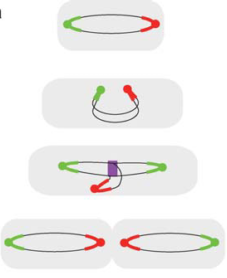
\includegraphics[scale=0.8]{./img/repl_simple.png}
	\end{center}
 \caption[Représentation schématique de la réplication du chromosome bactérien]{Représentation schématique de la réplication du chromosome bactérien. \\ Vert: \textit{ori}. Rouge: sites de terminaison. Violet: réplisome. Adapté de \citep{Ghosh2006}} \label{figRepl}
 \end{figure}
 
Dans la réplication de tout réplicon, trois phases peuvent être distinguées: 
\begin{description}
\item[$\bullet$] L'initiation qui correspond à l'ouverture de l'\textit{ori} par des protéines initiatrices.
\item[$\bullet$] L'élongation ou assemblage du brin néo-formé par les ADN-polymérases.
\item[$\bullet$] La terminaison qui est la relaxation des complexes de réplication pouvant s'accompagner de la résolution de dimère.
\end{description}
La réplication chez les chromosomes bactériens est conservée et suit globalement le modèle décrit chez \textit{E. coli}, alors qu'il existe trois types de réplication dans le cas des plasmides \citep{DelSolar1998}:
\begin{description}
\item[$\bullet$] la réplication thêta, similaire à la réplication chromosomique,
\item[$\bullet$] la réplication par rotation de cercle (RC),
\item[$\bullet$] la réplication par déplacement de brin (SD).
\end{description}
Parmi les plasmides à réplication de type thêta, on peut différencier les plasmides à itérons, sites spécifiques d'interaction avec les protéines Rep au niveau de leur \textit{ori}, et les plasmides de type ``DnaA-like" \citep{petersen2011origin}, des autres plasmides. \\
Les mécanismes et protéines majeurs impliqués dans la réplication, la ségrégation et le cycle cellulaire du génome bactérien sont résumés ci-dessous. La littérature existante fait majoritairement référence à quelques organismes modèles seulement, les principaux étant \textit{E. coli} (gamma-protéobactérie), \textit{Caulobacter crescentus} (alpha-protéobactérie) et \textit{Bacillus subtilis} (firmicute).\\


 \subsection{Origine et initiation de la réplication}\label{ori}
	Toutes les cellules des trois domaines de la vie possèdent des mécanismes de régulation contrôlant la réplication durant la phase d'initiation \citep{clark1967dna}. Les protéines majeures impliquées dans l'initiation de la réplication des réplicons sont présentées Table \ref{taboriini}. Sont ensuite détaillés la structure des origines de réplication, le déroulement et la régulation de l'initiation.
  
 \begin{longtable}{@{\hspace{-2cm}\hspace{1cm}} >{\bfseries}p{0.2\textwidth} | >{\small}p{0.9\textwidth}}
	 \caption{Principales protéines impliquées dans l'initiation de la réplication}
	 \label{taboriini}\\
	 \endfirsthead
	 DnaA & protéine s'attachant à l'ADN de façon spécifique. C'est un acteur principal de la cascade d'événements initiant la réplication des chromosomes bactériens et de certains plasmides \citep{petersen2011origin}. Ces événements incluent la reconnaissance de l'origine (\textit{ori}), son ouverture et l'attachement d'hélicases \citep{higgins2005bacterial}. DnaA est aussi un facteur de transcription \citep{Messer2002}. On estime que des homologues de DnaA existent chez toutes les espèces bactériennes \citep{yoshikawa1991structure,Messer2002}. \\
	\\[-0.2cm]
	DnaB & l'hélicase réplicative chez les bactéries. Elle est composée de six sous-unités et catalyse la séparation des brins de l'ADN \citep{o2013principles}. De même que pour DnaA, on considère que chaque organisme bactérien dispose d'une hélicase réplicative. Elle est de plus retrouvée dans les trois domaines du vivant.\\
	\\[-0.2cm]
	DnaC & paralogue de DnaA. C'est un facteur supplémentaire permettant l'attachement et la stabilisation de DnaB à \textit{ori} \citep{Mott2007}.\\
	\\[-0.2cm]
	IciA & (\textbf{Inhibitor} of \textbf{c}hromosome \textbf{i}nitiation) membre de la famille des facteurs de transcription LysR, très répandu chez les bactéries Gram négatif. IciA agit en tant qu'antagoniste de DnaA en inhibant l'initiation de la réplication au niveau d'\textit{ori} \citep{Dillon2010}.\\
	\\[-0.2cm]
	Rep & Cette dénomination fait référence de façon générique aux protéines impliquées dans l'initiation de la réplication des plasmides. Elles sont apparentées par leur séquence aux protéines impliquées dans la conjugaison (Tra et Mob) \citep{DelSolar1998} et sont retrouvées sur la plupart des plasmides dont la séquence complète a été réalisée. Elles peuvent comporter des domaines fonctionnels similaires \citep{DelSolar1998}, suggérant une origine commune. Tout comme DnaA avec le chromosome, les protéines Rep intéragissent avec les \textit{ori} plasmidiques par la reconnaissance de motifs spécifiques. La désignation “Rep” englobe les protéines initiatrices nécessaires pour les trois types de réplication plasmidique bien qu'elles puissent correspondre à des protéines différentes avec des fonctions distinctes. Généralement les plasmides de type thêta codent pour un seul initiateur protéique, RepA, TrfA ou RepE, qui active ou inhibe la réplication selon sa configuration (dimère ou monomère) \citep{Kruger2004}. Les plasmides de type SD codent pour trois protéines Rep: RepA (hélicase), RepB (primase) et RepC (facteur stabilisateur de l'hélicase de type DnaC) \citep{DelSolar1998}. Les Rep des plasmides de type RC sont très conservées, et contiennent deux domaines spécifiques: le domaine \textit{dso} de reconnaissance de l'origine et le domaine de coupure  \citep{khan2005plasmid}. Ces protéines possèdent un résidu tyrosine qui est impliqué dans la coupure de l'ADN \citep{khan2005plasmid}. Elles recrutent une hélicase de l'hôte, PcrA, qui possède des homologies avec l'hélicase Rep d'\textit{E. coli}.\\
	\\[-0.2cm]
	 DnaG & primase qui synthétise de courts fragments d'ARN, ou brins d'Okazaki, servant de points d'initiation pour la synthèse d'ADN \citep{o2013principles}.\\
	\\[-0.2cm]
	 Dam & (\textbf{D}NA \textbf{a}denine \textbf{m}ethylase) méthyle les motifs GATC au niveau de l'adénine et participe à la régulation de l'initiation.\\
	\\[-0.2cm]
	 SeqA & (\textbf{Seq}uestration \textbf{A} protein) régule l'initiation de la réplication en se fixant aux motifs GATC hémiméthylés au niveau d'\textit{ori}. L'origine néo-formée est ainsi séquestrée, empêchant un nouvel amorçage de la réplication par DnaA.\\
	\\[-0.2cm]
	 Hda & Homologue de DnaA. Elle intervient dans la régulation de DnaA chez \textit{E. coli}. Elle interagit avec l'ADN polymérase III, ce qui stimule l'activité de DnaA et contribue à l'ouverture de l'ADN au niveau d'\textit{ori}. Des orthologues de Hda ont été trouvés uniquement chez les gamma-protéobactéries \citep{zakrzewska2007regulation}. Chez \textit{B. subtilis}, c'est la protéine YabA qui joue ce rôle \citep{Mott2007}. \\
	\\[-0.2cm]
	 SSB & (\textbf{S}ingle \textbf{S}trand \textbf{B}inding proteins) En se fixant sur l'ADN mono-brin généré par l'ouverture de l'\textit{ori}, ces protéines stabilisent le complexe d'initiation \citep{o2013principles}.\\
	\\[-0.2cm]
	 DiaA & (\textbf{D}NA \textbf{i}nitiator-\textbf{a}ssociating factor) protéine découverte relativement récemment chez \textit{E. coli}. Elle se fixe à DnaA et est impliquée dans la synchronisation de l'initiation \citep{Katayama2010}. \\
	\\[-0.2cm]
	 CtrA & (\textbf{C}ell cycle \textbf{t}ranscriptional \textbf{r}egulator A) régulateur maître, caractérisé chez \textit{C. crescentus}. CtrA contrôle de nombreuses fonctions du cycle cellulaire et agit notamment sur les gènes \textit{ftsZ, ftsA} et \textit{ftsQ} (\textit{cf.} ci-après). Des homologues de CtrA semblent présents uniquement chez les alpha-protéobactéries \citep{Brilli2010,thanbichler2010}. \\
	\\[-0.2cm]
	 DivK & (cell \textbf{div}ision response regulator \textbf{K}) régulateur antagoniste de CtrA lorsque il est activé \citep{Brilli2010}.\\
	\\[-0.2cm]
	 YabA & inhibiteur de DnaA chez \textit{B. subtilis}. YabA forme un complexe avec DnaA et l'ADN polymerase III (\textit{cf.} ci-après) et limite le nombre de protéines initiatrices disponibles \citep{Katayama2010}. YabA est retrouvée chez d'autres bactéries Gram-positif \citep{Mott2007}.\\
	\\[-0.2cm]
	 SirA et Spo0A & (\textbf{S}porulation \textbf{i}nhibitor of \textbf{r}eplication protein \textbf{A} et \textbf{S}porulation stage  \textbf{0} protein \textbf{A}, respectivement) protéines impliquées dans la séquestration d'\textit{ori} chez \textit{B. subtilis} et ses proches voisins taxonomiques seulement.\\
	\end{longtable}
	
	
\subsubsection{Structure des origines de réplication}\label{oristruct}
\begin{description}
\item[$\blacktriangleright$] L'origine de réplication d'un chromosome bactérien typique est une courte séquence nucléotidique (250 pb chez \textit{E.coli}; Figure \ref{figoriecoli}), organisée en une région riche en Adénine et Thymine et en différents motifs structuraux \citep{Robinson2005,rajewska2012rich}.
\begin{figure}[H]
	\begin{center}
		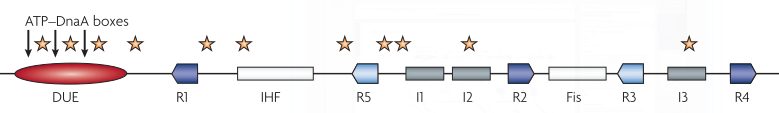
\includegraphics[width=0.9\linewidth]{./img/ori_schema.png}
	\caption[Structure de l'origine de réplication de \textit{E. coli}]{Origine de réplication de \textit{E. coli}.\\ DUE: DNA Unwinding Element, riche en bases A+T. R1, R2, R3, R4: boîtes DnaA orientées. Motifs présentant une affinité forte pour DnaA : bleu sombre, et faible: bleu clair. Rectangles blancs: sites de fixation de IHF et Fis. Étoiles: motifs GATC. Rectangles gris: sites I de fixation préférentielle de DnaA-ATP. Flèches: quatrième classe de motifs de fixation de DnaA-ATP exclusivement, dans DUE. Adapté de \citep{Mott2007}}\label{figoriecoli}.
	\end{center}
\end{figure} 
Sa proximité avec certains gènes engendre plusieurs systèmes de régulation. La plus importante interaction est avec DnaA, au niveau des boîtes DnaA qui structurent l'origine de réplication par leur type et leur orientation et permettent l'ouverture d'\textit{ori} au cours d'un changement de conformation lors de la fixation de DnaA \citep{Mott2007}. La région riche en bases A et T (DNA Unwinding Element; DUE) est le site d'ouverture proprement dit. Relativement moins d'énergie sera nécessaire à son ouverture de par sa richesse en paires A-T (2 liaisons covalentes) en comparaison à une région d'ADN comprenant des appariements G-C (3 liaisons covalentes). Cette région contient de plus, sur le chromosome d'\textit{E. coli}, trois 13-mères caractéristiques organisés en tandem, impliqués dans l'activité de DnaA \citep{Mott2007}. D'autres motifs structurels de cette région participent à la régulation de l'initiation, tels que les motifs d'attache de Fis et IHF et les motifs GATC. L'organisation des \textit{ori} des chromosomes d'autres bactéries présentent de nombreuses similarités avec l'\textit{ori} d'\textit{E.coli} et respectent la structure DUE + motifs spécifiques (boîtes DnaA, site de méthylation de Dam, etc) (Figure \ref{ori_div}). 
\end{description}

\begin{figure}[H]
		\begin{center}
			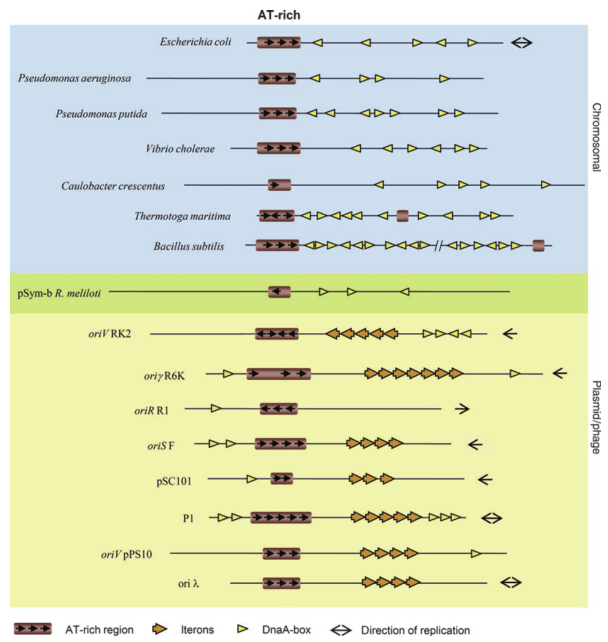
\includegraphics[height=0.5\textheight]{./img/ori_diversite.png}
			\caption[Diversité structurale des origines de réplication chez les bactéries]{Diversité des origines de réplication des réplicons bactériens chromosomiques et plasmidiques. Adapté de \citep{rajewska2012rich}. }\label{ori_div}
		\end{center}
\end{figure} 

\begin{description}
\item[$\blacktriangleright$] La structure des \textit{ori} plasmidiques présente certaines spécificités:
	\begin{description}
	\item[$\bullet$] La structure des \textit{ori} des plasmides à réplication thêta présente une organisation similaire à celles des chromosomes: DUE + motifs structuraux (Figure \ref{ori_div}). De nombreuses origines plasmidiques comportent des boîtes DnaA \citep{rajewska2012rich}, ce qui indique l'existence d'une interaction forte entre des régulateurs de l'hôte et la réplication plasmidique \citep{Kruger2004}. Les \textit{ori} plasmidiques peuvent également posséder des motifs spécifiques organisés en tandem, les itérons, qui permettent la fixation des protéines Rep et ainsi l'ouverture d'\textit{ori}. 
	\item[$\bullet$] L'origine de réplication chez les plasmides de type RC est un peu particulière car elle comporte deux origines: \textit{dso} (double strand origin) et \textit{sso} (single strand origin). La première est le lieu d'ouverture de l'ADN double brin. Elle comprend deux sites spécifiques: \textit{nick}, lieu de la coupure de l'ADN, et \textit{bind}, lieu de fixation de la protéine Rep. C'est à son niveau que s'amorce la réplication d'un des deux brins. L'autre origine, \textit{sso}, est l'endroit où est initiée la réplication de l'autre brin \citep{khan2005plasmid}. 
	\item[$\bullet$] Les plasmides SD sont majoritairement les plasmides de la famille IncQ \citep{Loftie-Eaton2012}. Leur origine est structurée en trois itérons correspondant au site de fixation de RepC, deux régions riches en G+C et A+T, respectivement, et deux sites d'initiation simple brin: \textit{ssiA} et \textit{ssiB} (\textbf{s}ingle \textbf{s}trand \textbf{i}nitiation A et B).
	\end{description}
\end{description}
  
\subsubsection{Déroulement de l'initiation}
\begin{description} 

\item[$\bullet$] Dans le modèle classique de l'initiation de la réplication du chromosome, l'attachement de plusieurs DnaA sur les boîtes DnaA d'\textit{ori} provoque une distorsion de l'ADN et conduit à son ouverture. Ce phénomène est suivi de la formation du complexe d'initiation (\textit{orisome}), et de l'action de l'hélicase sur l'ADN ouvert \citep{Robinson2005}. Chez \textit{E.coli}, Fis initialement présent est déplacé, ce qui permet la fixation de IHF et la formation d'un complexe protéique: le \textit{réplisome}  \citep{Mott2007,zakrzewska2007regulation}. L'ouverture est stabilisée par la fixation de protéines SSB qui protègent l'ADN simple brin.
\item[$\bullet$] L'initiation de la réplication thêta des plasmides est assez similaire à celle du chromosome bactérien: la fixation des protéines Rep sur les itérons provoque un changement de conformation de l'origine ce qui entraîne son ouverture. Des facteurs additionnels (DnaA, IHF, Fis, IciA, SeQ)  peuvent intéragir avec Rep ou se fixer à l'\textit{ori} afin de stabiliser/déstabiliser le complexe \citep{Kruger2004}.  
\item[$\bullet$] Chez les plasmides RC l'ouverture de l'ADN s'effectue au niveau du site \textit{nick} du site \textit{sdo} par fixation de la protéine Rep. Rep recrute ensuite une hélicase spécifique de l'hôte, PcrA (\textbf{P}lasmid \textbf{c}opy number \textbf{r}eduction protein \textbf{A}), qui étend l'ouverture. Un manteau de protéines SSB stabilise un des brins de l'ADN pendant que le complémentaire de l'autre brin est synthétisé par l'ADN polymérase III de l'hôte. La réplication du deuxième brin commence au site \textit{sso} et fait également intervenir la machinerie réplicative de l'hôte: ADN polymérase I et III, ADN gyrase et ADN ligase \citep{khan2005plasmid}.
\item[$\bullet$] L'initiation de la réplication des plasmides SD commence par la fixation de RepC au niveau des itérons, ce qui induit une rupture de la structure de l'origine et conduit à son ouverture. RepA pénètre alors dans l'ouverture et catalyse le déroulement de l'ADN. Lorsqu'ils sont à découvert, les sites \textit{ssiA} et \textit{ssiB} sont reconnus par RepB qui permet la fixation de l'ADN polymérase III et le début de la réplication grâce aux amorces synthétisées par RepB \citep{Loftie-Eaton2012}.
\end{description}
Contrairement à certains plasmides à réplication thêta, les plasmides SD et RC nécessitent une intervention réduite des protéines de l'hôte. Il est alors intéressant de constater qu'au final, \textbf{\color{orange} l'initiation de la réplication du chromosome n'est qu'un cas particulier de celle des plasmides thêta}.


\subsubsection{Régulation de l'initiation}
	Les modèles classiques de régulation de l'initation de la réplication impliquent majoritairement deux types de processus selon leur cible:
\begin{itemize}
	\item La séquestration, la déstabilisation ou l'occupation d'\textit{ori} et de ses motifs structuraux.
	\item L'inactivation, la séquestration ou la régulation des protéines initiatrices, Rep et DnaA.
\end{itemize}

\begin{description}
\item[$\blacktriangleright$] L'initiation de la réplication du chromosome est très précisément régulée pour garantir qu'une unique réplication du chromosome aura lieu au cours d'un cycle cellulaire.
	\begin{description} 
		\item[$\bullet$] Les mécanismes de séquestration de l'origine de réplication du chromosome chez \textit{E. coli} font intervenir les motifs GATC (GANTC chez \textit{B. subtilis}) et les protéines Dam qui méthylent ces sites au niveau de leur adénine. Avant initiation de la réplication, les sites GATC de l'origine sont doublement méthylés sur les brins direct et indirect (GATC étant un palindrome, si on considère son complémentaire). Juste après l'initiation, ces sites se retrouvent hémiméthylés car le brin néo-synthétisé n'a pas encore été soumis à l'action de Dam. Cette hémiméthylation conduit à la fixation de SeqA, ce qui empêche la fixation de DnaA au niveau de la nouvelle origine \citep{Mott2007,Kruger2004}. La séquestration de l'\textit{ori} par SeqA et Dam semble être une caractéristique des Entérobactéries, mais divers mécanismes de séquestration existent pour d'autres bactéries \citep{zakrzewska2007regulation}. Chez \textit{B. subtilis}, la séquestration d'\textit{ori} se fait par deux protéines non homologues de SeqA, Spo0A et SirA \citep{Katayama2010}.
		\item[$\bullet$]  La régulation de DnaA chez \textit{E.coli} implique aussi la titration des protéines au niveau d'une séquence caractéristique, le locus \textit{datA}, avec pour effet de réduire le nombre de DnaA actives disponibles.
		\item[$\bullet$]  Le mécanisme RIDA (Regulatory inactivation of DnaA) \citep{Mott2007} permet le passage de la forme active de DnaA, DnaA-ATP, à la forme inactive, DnaA-ADP, par l'intervention des protéines HdA et d'une des sous-unités de l'ADN polymérase III chez \textit{E. coli} \citep{Katayama2010}. Ces mécanismes semblent aussi exister chez d'autres bactéries \citep{zakrzewska2007regulation}.
		\item[$\bullet$]  DnaA a aussi un rôle de facteur de transcription en se fixant sur les promoteurs de certains gènes. Elle exerce aussi une auto-inhibition de sa synthèse en se fixant au promoteur de son gène \citep{zakrzewska2007regulation}.
	\end{description}
	
\item[$\blacktriangleright$] Différents mécanismes de régulation de l'initation sont spécifiques des plasmides.
	\begin{description} 
		\item[$\bullet$]  Des mécanismes de séquestration d'\textit{ori} existent également chez les plasmides. Un exemple en est le \textit{handcuffing} de l'origine de réplication des plasmides à réplication thêta et à itérons. Les \textit{ori} des deux plamides néo-formés se lient \textit{via} les protéines Rep fixées, empêchant leur accès \citep{Kruger2004}.
		\item[$\bullet$]  Le contrôle de la disponibilité en protéines Rep chez les plasmides  dépend notamment de l'auto-régulation de la transcription des gènes \textit{rep}. Il peut aussi passer par la structure-même de l'\textit{ori} qui peut titrer Rep grâce à ses itérons ou des sites annexes \citep{Kruger2004}. Certaines protéines initiatrices Rep, activatrices dans leur forme monomérique, peuvent former des dimères et alors devenir inhibitrices de la réplication \citep{Kruger2004,Cervantes-Rivera2011}. L'équilibre thermodynamique étant plutôt en faveur des dimères, l'introduction d'un plasmide dans un hôte qui abrite déjà un plasmide utilisant la même protéine Rep aura tendance à ne pas pouvoir se répliquer, l'initiation étant directement bloquée par les dimères de protéines Rep des plasmides présents. Ainsi les protéines Rep interviennent aussi dans les mécanismes dit d'“incompatibilité plasmidique”.
		\item[$\bullet$]  Des inhibitions par intervention d'ARN anti-sens agissant au niveau de la régulation de l'initiation plasmidique ont été caractérisées \citep{brantl2004plasmid}. L'inhibition intervient majoritairement dans le blocage de la traduction de l'ARNm des protéines activatrices Rep (par exemple, chez le plasmide R1 d'\textit{E. coli}) ou en se fixant au niveau de leurs cibles. Dans le cas des plasmides de type “RepABC”, le gène de l'activateur de l'initiation RepC étant inclus dans un opéron regroupant \textit{repA} et \textit{repB} (homologues de \textit{parA} et \textit{parB}, respectivement), la synthèse de RepC peut être pseudo-auto-inhibée par RepA et/ou RepB \citep{Pinto2012}, ou inhibée par un ARN antisens dont le gène est présent à l'intérieur même de l'opéron \citep{Cervantes-Rivera2011}. Enfin, de nombreuses protéines de l'hôte (DnaA, IHF, Fis) peuvent intervenir dans la régulation des gènes \textit{rep} ou participer à l'inactivation des protéines Rep, ainsi que dans l'activation/inactivation des \textit{ori} plasmidiques \citep{Kruger2004}. 
	\end{description}
\end{description}


\subsection{Élongation}
	Après la formation du replisome, l'ADN est répliqué bidirectionnellement chez les chromosomes et la majorité des plasmides à réplication thêta, et unidirectionnellement chez les autres, les plasmides à réplication RC et SD et certains plasmides à réplication thêta. Les protéines clé formant les complexes de réplication organisés aux deux fourches de réplication, sont les suivantes: 
\begin{itemize}
\item une hélicase faisant passer l'ADN du stade double-brin au stade mono-brin,
\item des molécules stabilisatrices de l'ADN mono-brin (SSB),
\item des primases synthétisant des amorces ARN nécessaires à la formation des fragments d'Okazaki,
\item des polymérases synthétisant l'ADN et/ou remplaçant l'ARN par de l'ADN,
\item des systèmes de correction d'erreur,
\item des ligases liant les différents fragments synthétisés.
\end{itemize}
	Deux types de protéines additionnelles sont nécessaires au bon fonctionnement des polymérases: des protéines d'attache à l'ADN (pinces), qui forment généralement un anneau glissant autour de l'ADN, et des protéines permettant l'établissement des protéines pinces sur l'ADN. Les principales protéines impliquées dans l'élongation sont présentées Table \ref{tabelongprot}. Une bonne revue des différents mécanismes moléculaires impliqués dans l'élongation peut être trouvée dans \citep{Johnson2005a}. 
  
\begin{longtable}{@{\hspace{-2cm}\hspace{1cm}} >{\bfseries}p{0.2\textwidth} | >{\small}p{0.9\textwidth}}
	\caption{Principales protéines impliquées dans l'élongation}\label{tabelongprot}\\
	\endfirsthead
	holoenzyme, \mbox{ADN} \mbox{polymérase III} & L'ADN polymerase III est un complexe comprenant différentes protéines (10 chez \textit{E. coli}), incluant les polymérases cœur, la pince glissante et cinq sous-unités responsables du chargement de la pince sur l'ADN. Ces protéines ont été plus particulièrement détaillées chez les bactéries Gram négatif (\textit{E. coli} surtout) mais semblent être retrouvées chez l'ensemble des bactéries ainsi que chez les Archées \citep{o2013principles}.\\
	Pol III core & Ces protéines interviennent dans les fonctions polymérase (\textbf{DnaE}) et 3'-5' exonucléase (\textbf{DnaQ}).\\
	\\[-0.2cm]
	DnaN & Pince circulaire de l'ADN polymérase III.\\
	\\[-0.2cm]
	Complexe d'attache de la pince & Chez \textit{E. coli}, cinq sous-unités sont responsables du chargement de la pince: \textbf{DnaX} (partie mobile), \textbf{HolA} (ouverture de la pince), \textbf{HolB} (partie fixe), \textbf{HolC} (protéine de transfert) et \textbf{HolD} (stabilisateur).\\
	\\[-0.2cm]
	PolA & ou ADN polymérase I. Enlève les amorces ARN par sa fonction exonucléase.\\
	\\[-0.2cm]
	DNA ligase I & Lie les fragments d'Okazaki en un seul fragment continu.\\
	\\[-0.2cm]
	GyrA et GyrB & protéines de type topoisomérase. Elles ont pour rôle de relaxer les superenroulements créés dans l'ADN lors de la réplication et par l'action des hélicases. Les topoisomérases peuvent être classées en deux catégories selon qu'elles agissent sur l'ADN double ou simple brin. GyrA et GyrB sont les deux sous-unités de la topoisomérase II d'\textit{E. coli} et agissent sur l'ADN double brin.\\
\end{longtable}

Une particularité de la réplication des plasmides SD, est qu'en plus d'être unidirectionnelle, il n'y a pas de production de fragment d'Okazaki pendant celle-ci. Les réplications SD et RC ont de plus la particularité de générer, durant la réplication, un intermédiaire d'ADN simple brin. Celui-ci étant hautement instable, ces types de réplication sont limités aux petits réplicons. 


\subsection{Terminaison de la réplication et résolution de dimère de réplicon}\label{ter}
 
\subsubsection{Mécanismes de terminaison de la réplication}
	Trois modèles décrivent actuellement la terminaison de la réplication des réplicons bactériens \citep{kono2012validation}:
\begin{itemize}
	\item le modèle \textbf{\textit{fork collision}} (collision de fourches) où la réplication bidirectionnelle s'interrompt lorsque les réplisomes des deux fourches de réplication se rencontrent. 
	\item le modèle \textbf{\textit{fork trap}} (piégeage de fourche) impliquant des associations ADN/protéine de type \textit{ter}/Tus qui entravent la progression de la polymérase à des sites spécifiques. Une protéine (Tus chez \textit{E. coli}, RTP (\textbf{R}eplication \textbf{T}erminaison \textbf{P}rotein) chez \textit{B. subtilis} \citep{kono2012validation}) se fixe sur l'ADN de façon site-spécifique et intéragit avec les protéines du réplisome afin de les déstabiliser \citep{kono2012validation,Johnson2005a}. 
	\item le modèle \textit{\textbf{dif-stop}}, contrairement aux deux précédents, implique une terminaison de la réplication à un site unique et précis.
 \end{itemize}
	Le modèle type \textit{ter}/Tus a été caractérisé pour le chromosome d'\textit{E. coli}. La région de la terminaison est bi-polarisée par une distribution de motifs \textit{ter}, orientés selon le sens de la réplication, de part et d'autre du site \textit{dif}. La protéine Tus n'est pas conservée dans le domaine bactérien et son homologue fonctionnel chez \textit{B. subtilis}, RTP, diffère tant au niveau structurel que par sa séquence, ce qui suggère une évolution relativement récente du modèle \textit{fork trap} \citep{kono2012validation}. 
	Les chromosomes ne possédant pas d'homologues fonctionnels des protéines \textit{Tus} (\textit{e.g.}, Firmicutes), ainsi que les plasmides à réplication thêta, semblent posséder un modèle d'arrêt de la réplication de type \textit{fork collision} \citep{kono2012validation}. Les plasmides se répliquant de façon unidirectionnelle n'utilisent pas d'appareil de terminaison ni ne suivent le modèle par collision de fourches.\\
Dans la terminaison de la réplication des plasmides de type RC, les protéines Rep semblent impliquées en promouvant une coupure de l'ADN au niveau du site d'ouverture \textit{dso}, ce qui libère un réplicon néo-formé ainsi qu'un intermédiaire simple brin \citep{,DelSolar1998,khan2005plasmid}. Chez les plasmides SD la réplication finit de même au site d'ouverture, la réplication étant monodirectionnelle \citep{Loftie-Eaton2012}.\\
	Les principales protéines jouant un rôle dans la terminaison de la réplication sont présentées Table \ref{tabrepelong}.

\begin{longtable}{@{\hspace{-2cm}\hspace{1cm}} >{\bfseries}p{0.2\textwidth} | >{\small}p{0.9\textwidth}}
	\caption{Principales protéines impliquées dans la terminaison de la réplication} \label{tabrepelong} \\
	\endfirsthead
	ParC & Sous-unité A de la topoisomérase IV. Trouvée chez \textit{E. coli} et \textit{B. subtilis} \citep{barnes2003dna}.\\
	\\[-0.2cm]
	ParE & Sous-unité B de la topoisomérase IV. Trouvée chez \textit{E. coli} et \textit{B. subtilis} \citep{barnes2003dna}.\\
	\\[-0.2cm]
	FtsK/SpoIIIE/ Tra & FtsK (\textbf{F}ilamenting \textbf{t}emperate \textbf{s}ensitive protein \textbf{K}; SpoIIIE chez \textit{B. subtilis)} Translocase essentielle impliquée dans le cycle cellulaire et coordonnant les dernières étapes de la cytokinèse chez \textit{E. coli} \citep{graham2010ftsk} en intéragissant avec \textbf{ParC} et \textbf{XerD} \citep{barre2000ftsk}. Sa structure héxamérique entoure l'ADN et interagit avec \textbf{FtsZ, FtsQ, FtsL} et \textbf{FtsI}, autres protéines impliquées dans le cycle cellulaire. Cette famille de translocases est très conservée chez les bactéries (sauf les Cyanobactéries) \citep{bigot2007ftsk}. \textbf{Tra}, translocase trouvée chez certains éléments mobiles et impliquée dans la conjugaison, appartient à la même famille protéique \citep{bigot2007ftsk}.\\
	\\[-0.2cm]
	Tus & Cette protéine se fixe sur les motifs \textit{ter} et déstabilise les protéines du réplisome lorsque celui-ci est à proximité d'un complexe Tus-\textit{ter}. Elle est présente chez \textit{E. coli} et quelques Entérobactéries proches. Ni Tus, ni \textit{ter} ne sont conservés parmi les chromosomes bactériens.\\
	\\[-0.2cm]
	\mbox{Recombinases} \mbox{site-spécifiques} & \textit{cf.} ci-dessous.
\end{longtable}

Une des caractéristiques essentielles des sites de terminaison de la réplication chez les bactéries est qu'ils sont directement liés aux mécanismes moléculaires impliqués dans la résolution de dimère de réplicon.

 
\subsubsection{Résolution de dimère au niveau du site de terminaison}\label{dimere}
	Au cours de la réplication des réplicons chromosomiques ou plasmidiques, des dimères peuvent apparaître, où les deux intermédiaires de réplication ne forment qu'une seule molécule \textit{via} des processus de recombinaison homologue \citep{Johnson2005a}. La formation d'un dimère altère non seulement la ségrégation active des chromosomes et plasmides, mais perturbe également la réplication. Un multimère ayant plusieurs origines de réplication aura tendance à être sur-répliqué, ce qui peut conduire à l'épuisement de l'espace et des ressources disponibles de l'hôte  \citep{hallet2004dna}. Dans le cas des plasmides, il y a multimérisation du plasmide jusqu'à ce que le nombre de molécules disponibles lors de la division cellulaire ne soit pas suffisante pour assurer sa stabilité \citep{summers1984multimerization}. Ces phénomènes ne sont pas marginaux; chez \textit{E. coli}, 10 à 15\% des réplications entraînent la formation de dimère \citep{perals2000functional}.\\
	La résolution de dimère de chromosomes ou de plasmides requiert l'intervention d'une machinerie moléculaire dédiée impliquant des recombinases spécifiques, dont les principales représentantes sont le couple de protéines XerC/XerD. Ces recombinases agissent au niveau d'un site spécifique (site \textit{dif} des chromosomes) situé au niveau de la région de la terminaison de la réplication. Pour les plasmides, il existe différentes familles de recombinases qui présentent des mécanismes distincts (détaillées plus loin). Les sites de recombinaison sont eux-aussi différents de ceux des chromosomes \citep{hallet2004dna}. Contrairement au processus de recombinaison homologue, les systèmes de résolution de dimère impliquent une seule étape de recombinaison site-spécifique, indépendamment du cycle cellulaire pour les plasmides \citep{hallet2004dna} ou faisant intervenir FtsK pour les chromosomes. \\
	Ces systèmes dédiés sont bien conservés parmi les chromosomes bactériens ainsi que pour de nombreux plasmides \citep{thomas2004}.

 
 \subsubsection{Décaténation des régions terminales par les topoisomérases}
	Un autre obstacle à la séparation réussie des deux réplicons néo-formés est l'enchevêtrement des deux régions terminales \citep{thanbichler2010}. Les mécanismes impliqués dans la décaténation des deux réplicons font aussi intervenir FtsK qui interagit directement avec ParC et ParE, les deux sous-unités de la topoisomérase IV, impliquée dans la résolution des super-enroulements. En stimulant l'interaction de ParC et ParE entre la fin de la réplication et la séparation des cellules, FtsK permet l'activation de la topoisomérase IV \citep{thanbichler2010}. 



 \section{Partition active des réplicons}\label{segreg}
	Après qu'un réplicon a été correctement répliqué, chacun des deux exemplaires obtenus doit être ségrégé dans une des deux cellules fille en formation. Cette ségrégation peut être passive comme, par exemple, dans le cas des petits plasmides à taux de copie élevé \citep{Ebersbach2005} où les réplicons sont transmis de façon aléatoire à l'une des cellules fille. Dans le cas des réplicons à faible taux de copie, de grande taille et/ou d'une relative importance pour la vie de la bactérie, des mécanismes moléculaires sont nécessaires pour assurer une ségrégation réussie et la stabilité du matériel génomique au cours des générations. Il existe de grandes similarités entre les différents systèmes moléculaires de \textbf{partition} permettant une ségrégation active, présents chez les réplicons bactériens \citep{funnell2004partition}. Les acteurs majoritaires de ces systèmes sont les protéines de type \textbf{ParA} (ParA-\textit{like}), \textbf{ParB} (ParB-\textit{like}), ainsi que la séquence de type centromérique \textit{\textbf{parS}}(Table \ref{protseg}).
	 
 \begin{longtable}{@{\hspace{-2cm}\hspace{1cm}} >{\bfseries}p{0.2\textwidth} | >{\small}p{0.9\textwidth}}
\caption{Principales protéines impliquées dans la ségrégation des réplicons}\label{protseg}\\
\endfirsthead
  MRP & protéine fixant l'ATP, impliquée dans la ségrégation des chromosomes. \\
	\\[-0.2cm]
 ParA/SopA/ ParM & Par commodité ces protéines seront désignées sous l'appellation: ParA-\textit{like} et les gènes les codant, \textit{parA-like}. Les protéines ParA-\textit{like} peuvent agir en tant que répresseurs des gènes \textit{parA} et/ou \textit{parB}. Ce sont des NTPases qui utilisent l'énergie libérée par hydrolyse de l'ATP et mettent en mouvement les réplicons par des phénomènes de polymérisation. Selon les ParA-\textit{like}, différentes configurations peuvent être prises par les polymères, bien que la conformation générale semble être similaire à celle des microtubules. Trois catégories de ParA-\textit{like} peuvent être distinguées: les \textit{Walker-A P-loop} ATPases (ParA, SopA; type I), les \textit{actin-like} ATPases (ParM;  type II) et les \textit{tubulin-like} ATPases (TubZ; type III) \citep{Mierzejewska2012,funnell2004partition}. Deux sous-types de ParA type I sont identifiés selon leur structure: Ia (ParA des plasmides F et P1) et Ib (protéines plus courtes) \citep{Passot2012}. Les ParA-\textit{like} de type II (ParM) ont la capacité de former des polymères avec une architecture très similaire à celle de l'actine chez les eucaryotes. Les ParA-\textit{like} de type III ont été caractérisées plus récemment chez des plasmides de \textit{Bacillus cereus} \citep{zheng2013evolution}. Ce sont des GTPase, analogues des tubulines des eucaryotes. Les ParA des chromosomes sont usuellement de type I à quelques exceptions près (\textit{E. coli} notamment). \textbf{MreB}, protéine de structure liée au cycle cellulaire et vraisemblablement remplaçant ParA chez \textit{E. coli}, est proche de ParM structurellement \citep{Mierzejewska2012}.\\
	\\[-0.2cm]
  ParB/SpoB/ ParR & Par commodité ces protéines seront désignées sous l'appellation ParB-\textit{like} et les gènes les codant, \textit{parB-like}. Dans les premières phases de la ségrégation des réplicons, ces protéines s'attachent à leur séquence centromérique respective, \textit{parS} (parfois appelée \textit{parC}), et promeuvent la polymérisation des ParA-\textit{like} \citep{funnell2004partition}. Les ParB-\textit{like} possèdent aussi un rôle dans la régulation des systèmes de partition. Surexprimées, ces protéines, dans certains cas, inhibent les gènes autour de \textit{parS} \citep{funnell2004partition}. Les ParB-\textit{like} peuvent aussi jouer un rôle dans l'accrochage des réplicons à la membrane bactérienne \textit{via} d'autres protéines intermédiaires \citep{Toro2010,Mierzejewska2012}.
 \end{longtable}
 
	Ce système de partition aurait un fonctionnement similaire à celui de l'appareil mitotique eucaryote \citep{Mierzejewska2012}. L'étape initiale de la ségrégation de deux réplicons néo-formés débute par la fixation de la protéine ParB-\textit{like} sur la séquence centromérique \textit{parS}. Une fois assemblé, ce complexe peut interagir avec la protéine ParA-\textit{like}. Pour être actives, ces dernières nécessitent l'action de l'ATP. Différentes structures peuvent être formées et différentes modalités de ségrégations mises en œuvre selon la protéine ParA-\textit{like} impliquée \citep{Mierzejewska2012,funnell2004partition}. Le modèle général semble néanmoins impliquer une polymérisation des ParA-\textit{like}, ce qui a pour effet de “pousser” les réplicons aux pôles opposés d'une manière analogue à celle des microtubules  chez les Eucaryotes \citep{Mierzejewska2012}. La régulation des systèmes de partition se fait d'une part par la dépolymérisation naturelle des ParA-\textit{like}, et d'autre part par une régulation des gènes \textit{parA} et \textit{parB}, généralement regroupés dans un même opéron. Cette régulation fait intervenir les protéines ParA-\textit{like} et ParB-\textit{like} (autorégulation) ou des protéines annexes liées au cycle cellulaire \citep{Mierzejewska2012,funnell2004partition,Pinto2012}. Outre le système parABS, d'autres systèmes moléculaires peuvent ségréger les chromosomes bactériens. MukB et SMC (deux analogues) semblent par exemple être impliqués dans la ségrégation des chromosomes de \textit{E. coli} et de \textit{B. subtilis}, respectivement \citep{Toro2010}. Le système parABS est retrouvé chez la très grande majorité des réplicons bactériens, ce qui est en faveur d'une émergence ancienne et unique, potentiellement existant dès l'origine des premiers réplicons. Ces systèmes constituent de fait un point clé de caractérisation parmi les propriétés fondamentales des réplicons.



\section{Maintenance des réplicons et intégration dans le cycle cellulaire}\label{regul}
	Il existe un lien logique des contrôles de la réplication et des systèmes de ségrégation des réplicons avec le cycle cellulaire. Les divers mécanismes de maintenance développés par les réplicons permettent d'optimiser, en terme de coût énergétique et d'efficacité (\textit{i.e.}, minimiser le taux de processus défectueux), leur réplication/ségrégation au sein de l'hôte et leur maintien dans l'espace et le temps à travers le cycle cellulaire (Table \ref{maintenance}). De nombreux mécanismes moléculaires impliqués dans la structure des réplicons interviennent de fait dans la maintenance des réplicons. Classiquement, la fin de la réplication des chromosomes doit être suivie d'un détachement réussi des régions terminales des deux chromosomes, de processus de partition/ségrégation et des phénomènes de condensation selon un ordre précis \citep{thanbichler2010}. 
\\
\begin{longtable}{@{\hspace{-2cm}\hspace{1cm}} >{\bfseries}p{0.2\textwidth} | >{\small}p{0.9\textwidth}}
	 \caption[Principales protéines impliquées dans la maintenance et le cycle cellulaire]{Principales protéines impliquées dans la maintenance et le cycle cellulaire des réplicons bactériens}\label{maintenance}\\
	 \endfirsthead
	 AcrA & fait partie d'un complexe protéique servant au transfert de diverses molécules à travers la membrane. C'est un acteur clé dans le cycle cellulaire \citep{lau2005cell}. Son inhibition influence directement le fonctionnement moléculaire des protéines du divisiome \citep{li2011targeting}\\
	\\[-0.2cm]
	 AmiC & est une protéine périplasmique clôturant la formation du divisiome \citep{vicente2006septum}. \\
	\\[-0.2cm]
	 EzrA & est un régulateur négatif de l'assemblage de l'anneau de FtsZ chez \textit{B. subtilis} \citep{yamanaka1996identification}.\\
	\\[-0.2cm]
	 Fic & (Filamentation induced by cyclic AMP protein) est une protéine inductrice du cycle cellulaire chez \textit{E.coli} \citep{kawamukai1989nucleotide}. Elle est aussi présente chez \textit{B. subtilis}.\\
	\\[-0.2cm]
	 FtsZ & Protéine majeure impliquée dans la formation du septum et dans la division cellulaire. FtsZ s'assemble en anneau à l'équateur de la cellule, ce qui permet, par un mécanisme de constriction, de couper la membrane \citep{thanbichler2010}. FtsZ, très conservée parmi les bactéries (à une exception: \textit{Chlamydia}, \citep{li2011targeting}), est également présente chez certaines Archées \citep{vicente2006septum}.\\
	\\[-0.2cm]
	  FtsA & Protéine intervenant avec \textbf{ZipA} dans la formation de l'anneau FtsZ \citep{vicente2006septum}.\\
	\\[-0.2cm]
	  ZipA & s'accroche à FtsZ \textit{in vitro} et aide à la stabilisation de l'anneau de FtsZ \textit{in vivo} \citep{li2011targeting}. Tout comme FtsB, FtsL et FtsN, ZipA n'est pas retrouvée chez certaines bactéries \citep{li2011targeting}.\\
	\\[-0.2cm]
	  ZapA & Protéine participant avec FtsA et ZipA à la formation de l'anneau FtsZ \citep{vicente2006septum}.\\
	\\[-0.2cm]
	 FtsB, FtsE, FtsI, FtsN, FtsQ, FtsW, FtsX & protéines intervenant, après FtsA/ZipA, dans la stabilisation de l'anneau FtsZ \citep{vicente2006septum}.\\
	\\[-0.2cm]
	 GidA & (Glucose inhibited division protein A) protéine quasiment universelle dans les génomes bactériens, influe sur la réplication \citep{kinscherf2002global}. Ces protéines possèdent un domaine fonctionnel de type méthyltransferase.\\
	\\[-0.2cm]
	 GidB & (Glucose inhibited division protein B) est une protéine possédant, comme GidA, un domaine fonctionnel de type méthyltransferase. Tout comme GidA, GidB est probablement impliquée dans le cycle cellulaire \citep{ogasawara1992genes}. On la trouve aussi bien chez \textit{B. subtilis} que chez \textit{E. coli}.\\
	\\[-0.2cm]
	 TrmFO & est une protéine de la même famille que GidA qui semble également impliquée dans la division cellulaire \citep{cicmil2008crystallization}. Elle est généralement trouvée chez les bactéries à Gram positif.\\
	\\[-0.2cm]
	 SepF & est une protéine conservée chez les bactéries à Gram positif. Elle interagit avec FtsZ (chez \textit{B. subtilis}) et joue un rôle significatif dans le développement du septum \citep{hamoen2006sepf}.\\
	\\[-0.2cm]
	SlmA & Protéine fixant l'ADN et inhibitrice de l'assemblage de FtsZ \citep{thanbichler2010}. SlmA, présente chez \textit{E. coli}, est très peu conservée parmi les bactéries. \textbf{Noc} est son homologue fonctionnel chez \textit{B. subtilis}.\\
	\\[-0.2cm]
	  SulA & est une protéine du système SOS (réparation sur épreuve) caractérisée chez \textit{E. coli}. Elle est aussi impliquée dans l'arrêt de la division cellulaire en interagissant avec FtsZ \citep{yamanaka1996identification}. \\ 
	\\[-0.2cm]
	 MinC & est un inhibiteur de la formation de polymères de FtsZ par oscillations rapides entre les pôles de la cellule \citep{thanbichler2010}. \\
	\\[-0.2cm]
	 MinD & agit en concert avec MinC en s'attachant à celle-ci afin d'empêcher la polymérisation de FtsZ \citep{thanbichler2010}. \\
	\\[-0.2cm]
	 MinE & est organisée en anneau autour de la membrane et déplace progressivement la position des complexes MinCD \citep{thanbichler2010}. \\
	\\[-0.2cm]
	 MreB & est homologue de l'actine et est essentiel dans le maintien de la forme de bâtonnet d'\textit{E. coli}. Son inactivation entrave sérieusement la ségrégation des chromosomes \citep{Ebersbach2005}. MreB s'associe avec MreC et MreD. Elle est trouvée chez l'ensemble des bactéries.\\
	 \\[-0.2cm]
	 MreC et MreD & sont impliquées, en interaction avec MreB, dans la maintenance de la structure en forme de bâtonnet de la cellule et dans la ségrégation des chromosomes \textit{E. coli} \citep{wachi1989new}.\\
	\\[-0.2cm]
	MukB & joue un rôle central dans la condensation et la ségrégation de l'ADN, et le cycle cellulaire d'\textit{E. coli} \citep{thanbichler2010,yamanaka1996identification}. Cette protéine forme un complexe avec \textbf{MukE} et \textbf{MukF} et interagit avec \textbf{FtsZ} et la topoisomérase \textbf{ParC}.\\
	\\[-0.2cm]
	\mbox{MukE et MukF} & interagit avec MukB. MukF et MukE interagissent ensemble \citep{yamanaka1996identification}. \\
	\\[-0.2cm]
	 SMC & (Structural Maintenance of Chromosome) est un analogue de MukB. Elle joue un rôle central dans la condensation du chromosome et est liée à ScpA et ScpB.\\
	\\[-0.2cm]
	 ScpA et ScpB & sont deux protéines auxiliaires du complexe SMC. Elles ont été découvertes chez les bactéries à Gram positif et chez les Archées \citep{thanbichler2010}. ScpA s'accroche à SMC et est stabilisée par ScpB. Des mutations sur ScpA provoquent le même effet que des mutations sur SMC \citep{thanbichler2010}.\\
	\\[-0.2cm]
	  DivIVA & caractérisée chez \textit{B. subtilis}, est une protéine majeure du cycle cellulaire. Elle intervient en intéragissant ave minCD et régule la formation du septum \citep{edwards1997bacillus}. Elle est de plus associée à RacA \citep{OSullivan2011}.\\
	\\[-0.2cm]
	 RacA & est une protéine d'ancrage chez \textit{B. subtilis}. Elle accroche \textit{ori} aux pôles de la cellule afin de préparer la division cellulaire. Elle est associée à DivIVA \citep{OSullivan2011}.\\
	\\[-0.2cm]
	 RodA & est une protéine impliquée dans la division et l'élongation cellulaire. Elle est décrite chez \textit{B. subtilis} et \textit{E. coli} \citep{henriques1998control}.\\
	\\[-0.2cm]
	 Systèmes PSK & (Post Segregational Killing) Véritable système d'“addiction génique”, ces complexes géniques interviennent de façon indirecte dans la stabilité et la maintenance d'un élément génétique (plasmide, séquence d'insertion, phage, transposon, complexe allélique...). Ces systèmes sont classiquement organisés en un gène codant une toxine et un gène codant une antitoxine avec éventuellement un gène régulateur. Une modification dans le système (perte de l'antitoxine, perte du système, gradient de concentration...) peut entrainer une concentration trop importante de la toxine et la mort cellulaire. Il existe une variété de systèmes PSK: \textbf{higBA, mazEF, relBE, HOK/SOK, vapXD, parDE, epsilon-zeta, ccd, Phd/Doc}... \citep{kobayashi2004genetic}.\\
 \end{longtable}
 
	Les mécanismes moléculaires de la division cellulaire impliquent la protéine FtsZ comme “fer de lance”. Chez \textit{E. coli}, FtsZ forme une structure polymérique en forme d'anneau dirigeant le processus de la division cellulaire \citep{thanbichler2010}. L'intervention de protéines additionnelles est souvent requise pour contrôler la position et la formation du \textit{divisiome} (système protéique impliqué dans la division) telles que le système Min (impliquant les protéines \textbf{MinC, MinD} et \textbf{MinE}) et \textbf{SlmA} (chez \textit{E. coli}), Noc (chez \textit{B. subtilis}) ou le système \textbf{MipZ} chez \textit{Caulobacter crecentus} \citep{Thanbichler2010}. Une quinzaine de protéines supplémentaires (notamment \textbf{FtsA, FtsB, FtsE, FtsI, FtsN, FtsQ, FtsW, FtsX, ZipA, ZapA et AmiC}) particulièrement bien conservées parmi les réplicons bactériens, sont recrutées dans la formation du septum \citep{vicente2006septum}. Chez les plasmides, la réplication, bien qu'asynchrone par rapport au cycle cellulaire, doit être régulée pour i) éviter une multiplication anarchique des plasmides et aboutir à un épuisement des ressources de l'organisme (“runaway replication” \citep{DelSolar1998}), ii) dupliquer le matériel génétique au bon moment au bon endroit et, de ce fait, adapter le cycle plasmidique au cycle cellulaire, et iii) être transmis équitablement aux deux cellules fille de l'hôte originel \citep{Pinto2012}. Différents mécanismes moléculaires spécifiques sont utilisés par les plasmides pour se maintenir à moindre coût, en adéquation avec leur nature non-essentielle, potentiellement égoïste et asynchrone par rapport au cycle cellulaire. Les mécanismes dits d'addiction plasmidique, ou \textit{Post-Segregational Killing} (PSK), très largement représentés chez les plamides, sont caractérisés par l'installation dans le génome d'un complexe génique impliqué dans la production d'une toxine et de son antitoxine correspondante. Toute modification du complexe provoque la mort de l'hôte \citep{mochizuki2006genetic}. Ces systèmes sont avantageux pour les plasmides d'un point de vue évolutif car ils garantissent le maintien des plasmides dans l'hôte les hébergeant. Ils sont aussi présents sur les chromosomes et permettent, par exemple, la stabilisation d'un complexe allélique \citep{mochizuki2006genetic}. De façon générale, il est intéressant de constater que l'évolution des génomes a gardé de tels systèmes géniques au comportement égoïste: outre le maintien de populations plasmidiques \citep{mochizuki2006genetic}, ces systèmes peuvent contribuer à la maintenance chromosomique, comme par leur implication dans la survie de populations bactériennes en situation de carence ou faisant face à des éléments génétiques intrusifs (phages, transposons...) \citep{kobayashi2004genetic}. Ces systèmes sont également la preuve que \textbf{\color{orange}l'évolution des génomes bactériens a adapté des systèmes plasmidiques dans les processus de maintenance chromosomique (ou inversement).}

\section{Mécanismes moléculaires de recombinaison, d'intégration et de transfert génétique}\label{recom}
	Les recombinaisons génétiques sont des phénomènes d'échange de fragments entre deux molécules d'ADN. Elles nécessitent l'action de diverses protéines et enzymes dont les recombinases. On distingue la recombinaison homologue où des brins d'ADN sont échangés entre molécules homologues, des recombinaisons dite “site-spécifiques” pour lesquelles les enzymes agissent seulement au niveau de sites présentant des motifs structuraux particuliers. Les recombinaisons homologues sont majoritairement impliquées dans les phénomènes de réparation de l'ADN chromosomique pendant la réplication, où un des brins d'une première molécule d'ADN (double-brin) va recombiner avec un brin d'une deuxième molécule d'ADN endommagée et servir de matrice à différentes enzymes afin de corriger la lésion \citep{perry1997microbiology, Barre2005}. Elles interviennent aussi dans différents processus moléculaires chez les phages \citep{Lopes2010}.\\
	Contrairement aux processus de recombinaison homologue, les recombinaisons site- spécifiques sont réalisées par une machinerie moléculaire relativement simple où les recombinases vont prendre en charge les étapes de césure, d'échange et de fermeture de l'ADN \citep{hallet2004dna}. Elles ont lieu sur de courts segments d'ADN, les \textit{sites de recombinaison}. Les recombinaisons site-spécifiques interviennent notamment dans la résolution de dimère précédemment abordée, mais aussi, de façon très similaire, dans la réplication de certains transposons \citep{hallet2004dna}. Enfin, elles peuvent intervenir dans les processus d'intégration et d'excision des bactériophages et de différents éléments mobiles \citep{hallet2004dna}. 
 
 \subsection{Résolvases impliquées dans la résolution de dimère de réplicon}
	Plasmides et chromosomes, dans leur grande majorité, codent des systèmes protéiques de recombinaison homologue spécifiques à la résolution des dimères formés lors de la réplication. Les enzymes impliquées sont des \textbf{résolvases}. On en distingue deux familles: les tyrosine- et les sérine-recombinases (Table \ref{resolvases}). Cette distinction repose sur la nature de l'acide aminé servant en premier à l'attaque nucléophile de l'ADN par la recombinase.
\\
\begin{longtable}{@{\hspace{-3cm}\hspace{1cm}} >{\bfseries}p{0.3\textwidth} | >{\small}p{0.9\textwidth}}
\caption{Résolvases impliquées dans la résolution de dimère}\label{resolvases}\\
\endfirsthead
	Tyrosine-recombinases & Les tyrosine-recombinases présentent différents niveaux de complexité. Leur fonctionnement ne nécessite qu'un simple site de recombinaison ou peut impliquer des sites d'attache de protéines régulatrices. On trouve parmi elles les résolvases de type \textbf{Xer} qui sont un parfait exemple de protéine multi-usage, à mécanisme simple, et largement répandues parmi des plasmides et chromosomes bactériens. Le système Xer le mieux décrit fait intervenir deux protéines, \textbf{XerC} et \textbf{XerD}, qui effectuent la recombinaison homologue des réplicons au niveau du site \textit{dif}. Des homologues de ces protéines sont trouvés dans le génome de presque toutes les bactéries et archées ayant un chromosome circulaire \citep{hallet2004dna}\citep{cortez2010evidence}) et chez de nombreux plasmides, ce qui suggère une conservation stricte du système Xer/\textit{dif} pour les chromosomes bactériens \citep{Carnoy2009,Kono2011}. Il existe cependant des variations mono-protéiques au système XerCD. Dans le génome des firmicutes, une seule protéine homologue à XerC et XerD, \textbf{XerS}, fait office de résolvase \citep{Leroux2011}. Un autre système Xer chez une partie des epsilon-protéobactéries implique une unique recombinase, \textbf{XerH}, qui ne présente pas de lien phylogénique apparent avec XerS \citep{Carnoy2009}. Le système Xer/\textit{dif} n'est cependant pas présent de manière universelle. Certains génomes, principalement chez des endosymbiotes, ne semblent pas posséder de sites \textit{dif}, ni de protéines Xer \citep{Carnoy2009,Kono2011}. D'autres systèmes de recombinaisons, faisant notamment intervenir des sérines-recombinases, peuvent remplacer les systèmes Xer/\textit{dif} \citep{Carnoy2009}. Des résolvases différentes de la famille Xer peuvent exister et participer à la résolution des dimères chez certains plasmides, comme par exemple, les résolvases de la famille de ResD découvert chez un plasmide d'\textit{E. coli} \citep{hallet2004dna}. Enfin, les systèmes Xer/\textit{dif} chromosomiques fonctionnent différemment de ceux des plasmides. Ils requièrent l'intervention de protéines supplémentaires (FstK entre autres, \textit{c.f.} \ref{recom}) les liant au cycle cellulaire. \\
	\\[-0.2cm]
	Sérine-recombinases & Elles sont présentes sur les plasmides des bactéries à Gram positif ou négatif. Elles sont homologues des résolvases impliquées dans l'insertion de transposons et en sont clairement dérivées, pouvant d'ailleurs se substituer à celles de ces derniers \citep{hallet2004dna}. Le site de recombinaison est généralement proche des gènes codant les recombinases, ce qui facilite le transfert latéral d'un système fonctionnel. On en distingue plusieurs sous-familles: les recombinases de type Mu (proches des protéines du bactériophage Mu), de la famille Tn3 et les bêta-recombinases codées par certains plasmides de bactéries à Gram positif \citep{hallet2004dna}.
\end{longtable}
 
	Les chromosomes bactériens circulaires codent des tyrosine-recombinases, dont la grande majorité appartient au système XerC/XerD. Des homologues de ces protéines ont été identifiés chez de nombreux plasmides ainsi que chez des archées à génome circulaire \citep{hallet2004dna}. Les génomes linéaires ont des systèmes protéiques particuliers impliqués dans la résolution des télomères. Ces enzymes, les \textbf{ResT}, possèdent peu d'homologie de séquence avec les tyrosine-recombinases \citep{chaconas2005replication}. Les systèmes de résolution de dimère semblent avoir des fonctions annexes dans de nombreuses situations. Par exemple, ils peuvent être détournés par les phages pour s'insérer dans le génome de l'hôte ou permettre la conjugaison de leur génome \citep{Das2013,hallet2004dna} .
 
 
\subsection{Les autres recombinases}\label{parmge}
	Les familles des tyrosine- et sérine-recombinases incluent par ailleurs les “\textbf{transposases}”, impliquées dans l'insertion/excision des transposons, les “\textbf{relaxases}”, initiatrices de la réplication (Rep) et de la mobilisation (Mob) des plasmides RC, les “\textbf{intégrases}”qui catalysent les étapes d'intégration des rétrotransposons et rétrovirus, et certaines topoisomérases (Table \ref{MGE}). De manière générale, ces protéines catalysent des opérations d'excision/intégration de l'ADN et tiennent une place capitale dans les cycles des différents éléments génomiques mobiles (ou MGE pour \textit{Mobile genetic element}). 

\begin{longtable}{@{\hspace{-3cm}\hspace{1cm}} >{\bfseries}p{0.3\textwidth} | >{\small}p{0.9\textwidth}}
	\caption{Les recombinases distinctes des résolvases}\label{MGE}\\
	\endfirsthead
	DDE transposases & Ce sont des enzymes impliquées dans les cycles des transposons bactériens. L'action catalytique de ces enzymes impliquent trois acides aminés (Asp (D), Asp (D) et Glu (E), formant le motif DDE), qui coordonnent les transferts de groupement phosphoryle lors de la transposition \citep{higgins2005bacterial}. Ces transposases sont aussi présentes sur certains rétrovirus et rétrotranspons d'eucaryotes.\\
	\\[-0.2cm]
	Intégrases et transposases de type tyrosine-recombinase & Le système Cre/\textit{loxP} est un système de recombinaison trouvé chez le bactériophage P1 d'\textit{E. coli}. Il implique une unique recombinase \textbf{Cre} proche de l'intégrase \textbf{Int} du bactériophage lambda. Ce système est impliqué dans la circularisation des phages \citep{hallet2004dna}. Les tyrosine-recombinases comportent de plus des transposases codées par des transposons: Y2 ou RCT (pour Rolling Circle Transposition) \citep{higgins2005bacterial}, proches des protéines Rep des plasmides RC \citep{cornet2004non}, et les transposons Y codant une transposase plus classique.\\
	\\[-0.2cm]
	Intégrases et transposases de type sérine-recombinase & Plusieurs sérine-recombinases sont présentes en tant que transposases chez les transposons S \citep{higgins2005bacterial}. Tout comme pour les tyrosine-transposases, le site de transposition est moins contraint que le site de résolution \citep{cornet2004non}. Les intégrases des sérine-recombinases sont représentées par Hin et Gin, deux enzymes plasmidiques \citep{cornet2004non}. \\ 
	\\[-0.2cm]
 Relaxases & Cette famille hétéroclite d'enzymes regroupe en particulier les protéines qui se fixent sur le site de conjugaison des éléments conjugatifs et mobilisables, \textit{oriT}, et procèdent à son ouverture \citep{Guglielmini2013}. Ces protéines sont longues et comportent deux, ou plus, domaines fonctionnels (un domaine relaxase et un domaine hélicase). Différentes familles de relaxases sont identifiables et peuvent servir à classer les éléments conjugatifs \citep{Guglielmini2013}. Ces relaxases sont de plus structurellement homologues des protéines initiatrices de la réplication de type RC \citep{Smillie2010}.
\end{longtable}
 
 
\subsection{Les éléments transposables}\label{transposon}
	Les processus de recombinaison spécifique sont fortement impliqués dans les processus de ségrégation et de maintenance des réplicons bactériens. Ils sont à la base de la définition d'une classe d'éléments génétiques distincte des réplicons, les transposons (Table \ref{transposon}), bien que le type de recombinaison manifesté par les transposons diffère de la recombinaison site-spécifique impliquée dans la résolution de dimère de chromosome ou de plasmide. Différentes nomenclatures et types de transposons ont été définis selon leurs mécanismes d'insertion, les transposases impliquées, leurs sites d'insertion ou l'organisation de la séquence transposable \citep{Roberts2008, higgins2005bacterial}. 


\begin{longtable}{@{\hspace{-2.5cm}\hspace{1cm}}p{0.35\textwidth} | p{0.8\textwidth}}
	\caption{Principaux types de transposons}\label{transposon}\\
	\endfirsthead
	\textbf{Séquences d'insertion (IS)} & ou transposons unitaires. Ces séquences sont uniquement composées des structures (site de recombinaison) et gènes (transposases) impliqués dans la transposition.\\
	\\[-0.2cm]
	\textbf{Transposons composites} & sont composés d'IS et de gènes et structures additionnels codant, par exemple, des protéines de résistance aux antibiotiques.\\
	\\[-0.2cm]
	\textbf{Transposons conjugatifs} & ou ICE (\textit{Integrative Conjugative Element}) portent des gènes codant des fonctions d'excision et d'intégration (transposases/intégrases) et des fonctions de conjugaison \citep{Wozniak2010}.\\
	\\[-0.2cm]
	\textbf{Transposons mobilisables} & ou IME (pour \textit{Integrative Mobilisable Element}) peuvent être mobilisés entre cellules bactériennes, et codent en général leurs propres transposases \citep{Roberts2008}.\\
	\\[-0.2cm]
	\textbf{Îlots génomiques mobiles} & sont des séquences intégrées dans les génomes, codant leurs propres transposases, mais pas les gènes impliqués dans leur transfert inter-cellulaire. Ils contiennent des gènes modifiant le phénotype cellulaire (par exemple, îlots de pathogénicité) \citep{Boyd2009}.\\
	\\[-0.2cm]
	\textbf{Prophages transposables} & sont des génomes de bacteriophage intégrés dans des génomes bactériens et capable d'excision/insertion.\\
	\\[-0.2cm]
	\textbf{Prophages satellites} & sont des prophages déficients intégrés dans des génomes bactériens. Ils nécessitent l'intervention de la machinerie moléculaire d'autres prophages pour compléter leur cycle de réplication.\\
 \end{longtable}
 
 
	Ces éléments sont capables de s'insérer, en tant que fragments d'ADN discrets et non permutables, à différents sites dans les génomes \citep{higgins2005bacterial}. Par opposition aux réplicons, les éléments transposables ne sont pas capables de se maintenir et de se répliquer indépendamment de leur génome hôte. La transposition requiert l'action de transposases (\textit{c.f.} \ref{MGE}) qui catalysent les différentes réactions de coupure/jointure de l'ADN. Même si originellement les transposons ont été décrits comme codant des DDE transposases, une grande variété de transposons codent des transposases de type sérine- ou tyrosine-recombinase, dont certaines sont homologues des relaxases et des protéines Rep des réplicons RC \citep{Roberts2008}. Les transposons peuvent être soumis à des mécanismes de régulation contrôlant leur cycle d'excision/intégration, évitant de potentiels effets délétères à leur hôte. Ces mécanismes peuvent faire intervenir des ARN anti-sens, des protéines de méthylation (\textit{i.e.} Dam), des represseurs transcriptionnels ou des protéines de type NAP de l'hôte \citep{cornet2004non}. L'existence sur des ICE d'analogues de systèmes de partition a également été rapporté \citep{Wozniak2010}. 

 
 \subsection{Conjugaison des éléments génomiques} \label{conj}
	Un des derniers aspects de la description du matériel génomique bactérien concerne les mécanismes et structures impliqués dans la mobilisation des différents éléments génomiques. La \textbf{conjugaison} bactérienne est un des processus de dissémination de gènes entre cellules indépendamment de la reproduction \citep{lawley2004bacterial}. Elle implique le transfert d'ADN de cellule à cellule par contact avec établissement du canal de conjugaison, veritable “pont” moléculaire traversant les membranes cellulaires. Ce phénomène initialement décrit comme une spécificité plasmidique, a ensuite été caractérisé chez les ICE \citep{Wozniak2010}. Les systèmes de conjugaison sont constitués de trois sous-systèmes essentiels \citep{lawley2004bacterial,Smillie2010}:
\begin{itemize}
	\item Le transférosome (système de sécrétion de type IV: T4SS) qui est responsable de la déstabilisation de l'enveloppe cellulaire et de la synthèse du pilus.
	\item Le relaxosome, complexe protéique qui agit sur l'ADN au niveau de l'origine de transfert \textit{oriT}. Les enzymes du relaxosome sont responsables de l'ouverture du plasmide au site \textit{oriT} et du désenroulement de l'ADN grâce à des hélicases.
	\item Les protéines de couplage (T4CP) qui s'accrochent au transférosome et intéragissent avec la relaxase.
 \end{itemize}

	La conjugaison suit les étapes suivantes \citep{lawley2004bacterial}: i) Synthèse d'un pilus par la cellule donneuse et son intéraction avec la membrane de la cellule receveuse, suivie de la création d'un canal entre les deux membranes (\textit{mating pair formation}). ii) Intervention du relaxosome (et en particulier de la relaxase), qui coupe l'ADN de l'élément conjugatif au site \textit{nick}. Un des deux brins est alors “déroulé” et passe dans la cellule receveuse. iii) La réplication des deux molécules d'ADN simple brin dans les cellules par les machineries moléculaires des hôtes.\\
	La réplication des éléments conjugatifs est homologue à celle des plasmides de type RC. On distingue les éléments conjugatifs codant leur propre système T4SS, des éléments mobilisables possédant \textit{oriT}, relaxases et éventuellement un système T4CP \citep{Smillie2010}. Ces derniers peuvent être mobilisés et transférés à des cellules receveuses \textit{via} les systèmes T4SS et T4CP d'autres éléments conjugatifs.\\ 
	Il est remarquable que des modules fonctionnels d'ADN liés à la conjugaison et reliés d'un point de vue évolutif se retrouvent sur des plasmides de bactéries Gram-positif et Gram-négatif, ainsi que sur des transposons de type ICE et IME \citep{Francia2004}. De même, l'homogénéité relative des séquences \textit{oriT} identifiés sur certains plasmides et sur les ICE chez les bactéries Gram-positif et Gram-négatif suggère une origine ancienne \citep{Francia2004}. Ces homologies suggèrent que ces éléments génétiques ont évolués à partir d'un groupe de gènes et/ou de motifs d'ADN ancestraux qui ont divergé en s'adaptant à des situations particulières \citep{Francia2004}. 
 
 
 \section{Fluidité du matériel génétique}\label{parevoldesrepl}

“\textit{Rather than being a well-designed blueprint, a genome appears to be a temporary community of potentially mobile genes that essentially act selfishly}” \citep{mochizuki2006genetic}.\\\\

	Les différentes structures génomiques bactériennes et la relative diversité des mécanismes moléculaires impliqués dans les réplication, ségrégation et maintenance du génome laissent entrevoir la plasticité du génome bactérien. Les génomes sont soumis à des processus de modification et de transfert d'ADN internes, faisant intervenir un ou plusieurs éléments génétiques et réplicons, ou externes, impliquant plusieurs génomes bactériens (ou un génome et de l'ADN extra-cellulaire). Les échanges inter-génomiques sont généralement rassemblés sous la désignation de \textbf{T}ransfert \textbf{H}orizontal de \textbf{G}ènes (THG) et regroupent les processus de conjugaison (introduit dans la partie précédente), de transduction \citep{miller2004bacteriophage}, de transformation \citep{miller2004microbial}, ou encore les \textit{Gene Transfer Agents} plus récemment décrits. Les THG tiennent une part très importante dans l'évolution des génomes bactériens \citep{Wiedenbeck2011} et font intervenir des mécanismes moléculaires liés à la réplication, ségrégation et maintenance du génome. Ces mécanismes tiennent donc une place centrale dans la définition et l'évolution des génomes, notamment pour ce qui est de l'intégration et de la stabilisation dans l'organisme bactérien des différents éléments génomiques. Les mécanismes de recombinaison, en particulier, interviennent largement dans les échanges et inversions entre éléments génomiques. Les homologies structurelles et fonctionnelles partagées par les différentes classes de recombinases montrent des similitudes et indiquent de probables origines communes à ces molécules. Il semble de plus que l'on retrouve ces similitudes de manière plus générale (par exemple, avec les systèmes Par ou les systèmes conjugatifs). \textbf{Ainsi se dessine une continuité entre les différents réplicons et éléments génétiques retrouvés chez les bactéries ainsi que parmi les mécanismes moléculaires à l'œuvre dans leur maintenance.}	
 
\iffalse
\fi
 
